\section{Техническое задание}

\subsection{Основание для разработки}

Основанием для разработки является задание на выпускную квалификационную работу бакалавра <<Разработка веб-платформы для автоматизации бизнес-процессов управления персоналом компании>>. Проект реализуется в рамках производственной практики студента в компании ООО <<ВТИ-Сервис>>.

\subsection{Цель и назначение разработки}

Целью проекта является разработка и внедрение веб-платформы, которая обеспечит эффективное управление внутренними коммуникациями и координацией персонала.

Задачи разработки включают:

\begin{itemize}
  \item создание единого доступа ко всем внутренним бизнес-сервисам;
  \item централизация данных и снижение фрагментированности инструментов;
  \item повышение прозрачности процессов и контроль выполнения задач;
  \item ускорение документооборота и взаимодействия между сотрудниками;
  \item внедрение интуитивного интерфейса и адаптивной архитектуры.
\end{itemize}

\subsection{Функциональные задачи}

Разрабатываемая веб-платформа включает следующие сервисные модули:

  \textbf{Почта} — модуль для внутренней и внешней переписки. Реализует:
  \begin{itemize}
    \item просмотр и отправку писем;
    \item вложения и черновики;
    \item фильтрацию, сортировку и интеграцию с контактами.
  \end{itemize}

  \textbf{Контакты} — централизованная адресная книга:
  \begin{itemize}
    \item отображение статуса и информации о сотрудниках;
    \item быстрый доступ к действиям (сообщение, задача, звонок).
  \end{itemize}

  \textbf{Проекты} — система для постановки и отслеживания задач:
  \begin{itemize}
    \item создание задач и контроль сроков;
    \item фильтрация по статусу и исполнителям;
    \item иерархия задач и связь с календарём.
  \end{itemize}

  \textbf{Файлы} — облачное хранилище для документов:
  \begin{itemize}
    \item загрузка и скачивание;
    \item управление правами доступа;
    \item история изменений.
  \end{itemize}

  \textbf{Календарь} — модуль планирования событий:
  \begin{itemize}
    \item создание событий и напоминаний;
    \item интеграция с задачами и ВКС;
    \item уведомления о событиях.
  \end{itemize}

  \textbf{Разговоры} — встроенный мессенджер:
  \begin{itemize}
    \item чат с сотрудниками;
    \item групповые обсуждения;
    \item уведомления и синхронизация с почтой.
  \end{itemize}

  \textbf{ВКС} — видеоконференцсвязь:
  \begin{itemize}
    \item создание и участие во встречах;
    \item демонстрация экрана;
    \item чат во время звонков.
  \end{itemize}

  \textbf{Настройки} — модуль управления профилем:
  \begin{itemize}
    \item редактирование профиля;
    \item смена темы, языка;
    \item конфиденциальность.
  \end{itemize}

  \textbf{Панель управления} — стартовая страница с виджетами:
  \begin{itemize}
    \item отображение актуальных данных со всех сервисов;
    \item настройка отображаемых виджетов;
    \item персонализация интерфейса.
  \end{itemize}

\subsection{Требования пользователя к интерфейсу веб-платформы}

Интерфейс должен обеспечивать:
\begin{itemize}
  \item интуитивную навигацию между модулями;
  \item адаптивную вёрстку для десктопов и мобильных устройств;
  \item визуальное разграничение ролей пользователей;
  \item поддержку светлой и тёмной темы.
\end{itemize}

Композиция интерфейса сервиса <<Почта>> представлена на рисунке \ref{templ:image1} и состоит из:
\begin{itemize}
  \item кнопки для отправки письма(1);
  \item списка папок (2);
  \item окна для просмотра писем из выбранной папки (3);
  \item компонента пагинации (4);
  \item компонента навигации по сервисам (5);
\end{itemize}
\begin{figure}[H]
	\centering
	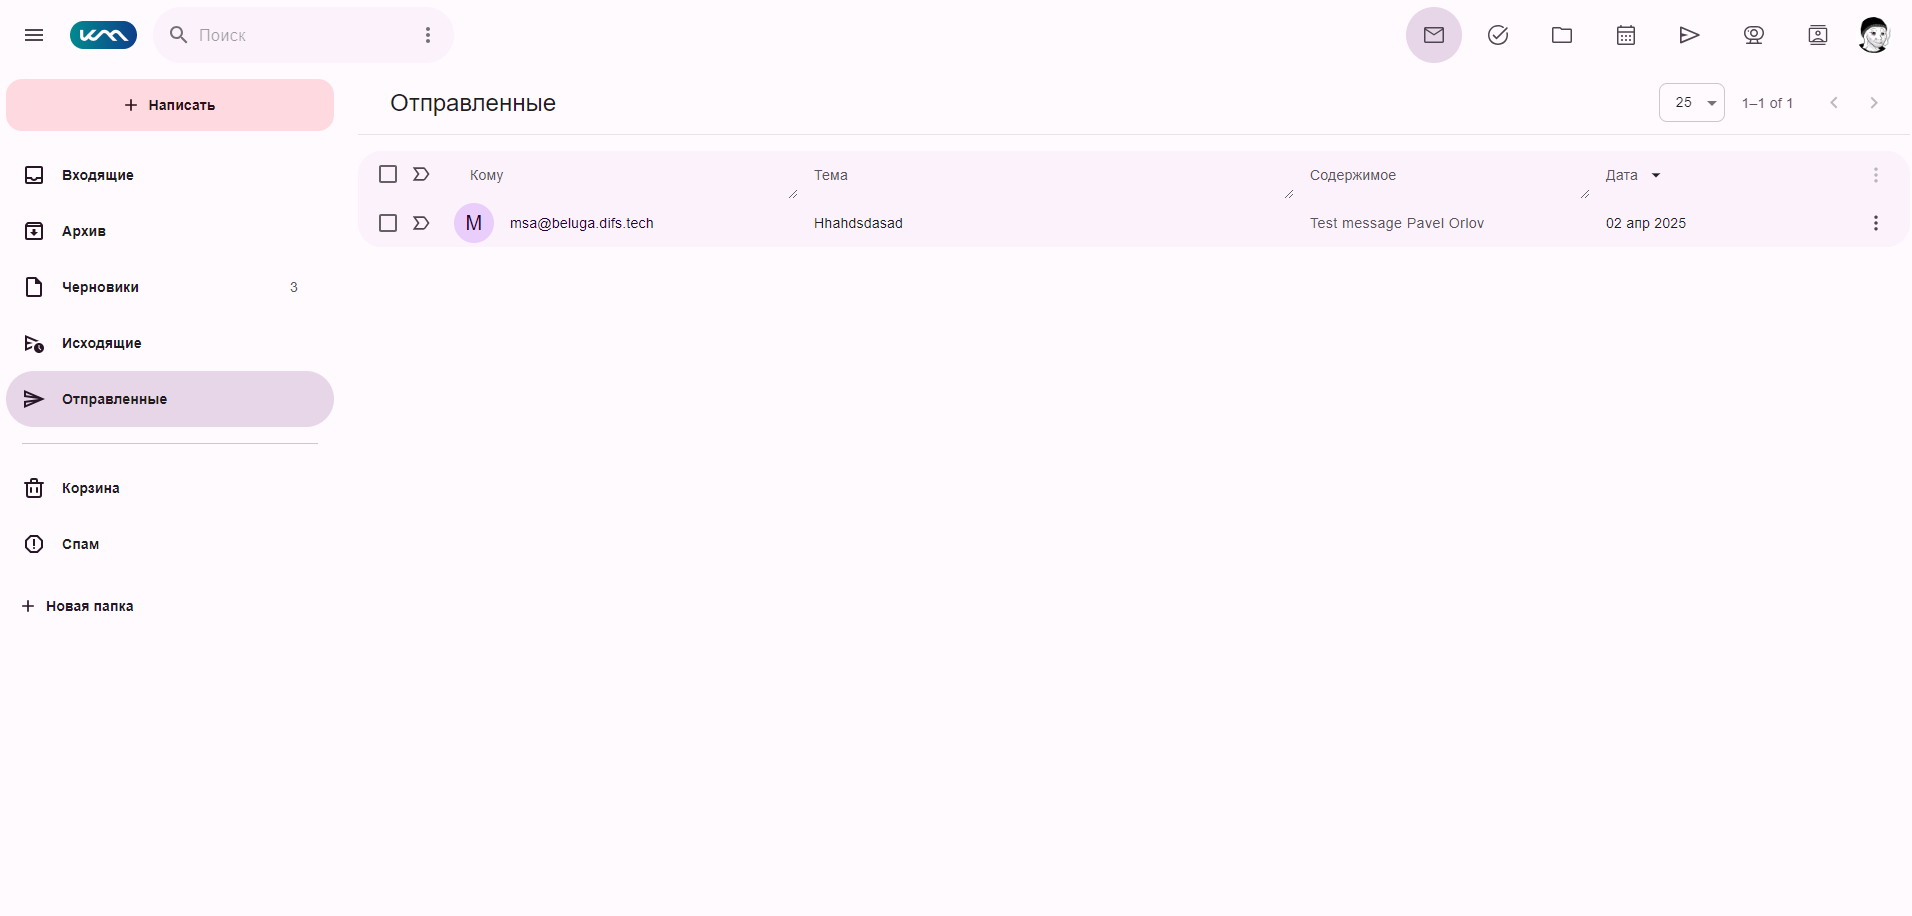
\includegraphics[width=1\linewidth]{images/почта}
	\caption{Композиция интерфейса сервиса <<Почта>>}
	\label{templ:image1}
\end{figure}

Композиция интерфейса написания письма в сервисе <<Почта>> представлена на рисунке \ref{templ:image1b} и состоит из:
\begin{itemize}
  \item окна ввода письма (1);
  \item поля ввода адресата (2);
  \item кнопок для ввода адресата с целью получения копии/скрытой копии (3);
  \item поля для ввода темы письма (4);
  \item окна для ввода тела письма (5);
  \item кнопок для отправки/сохранения письма в черновик (6);
  \item кнопок для прикрепления файла с компьютера или из сервиса <<Файлы>> (7);
  \item кнопки для закрытия окна без сохранения письма в черновик (8);
\end{itemize}
\begin{figure}[H]
	\centering
	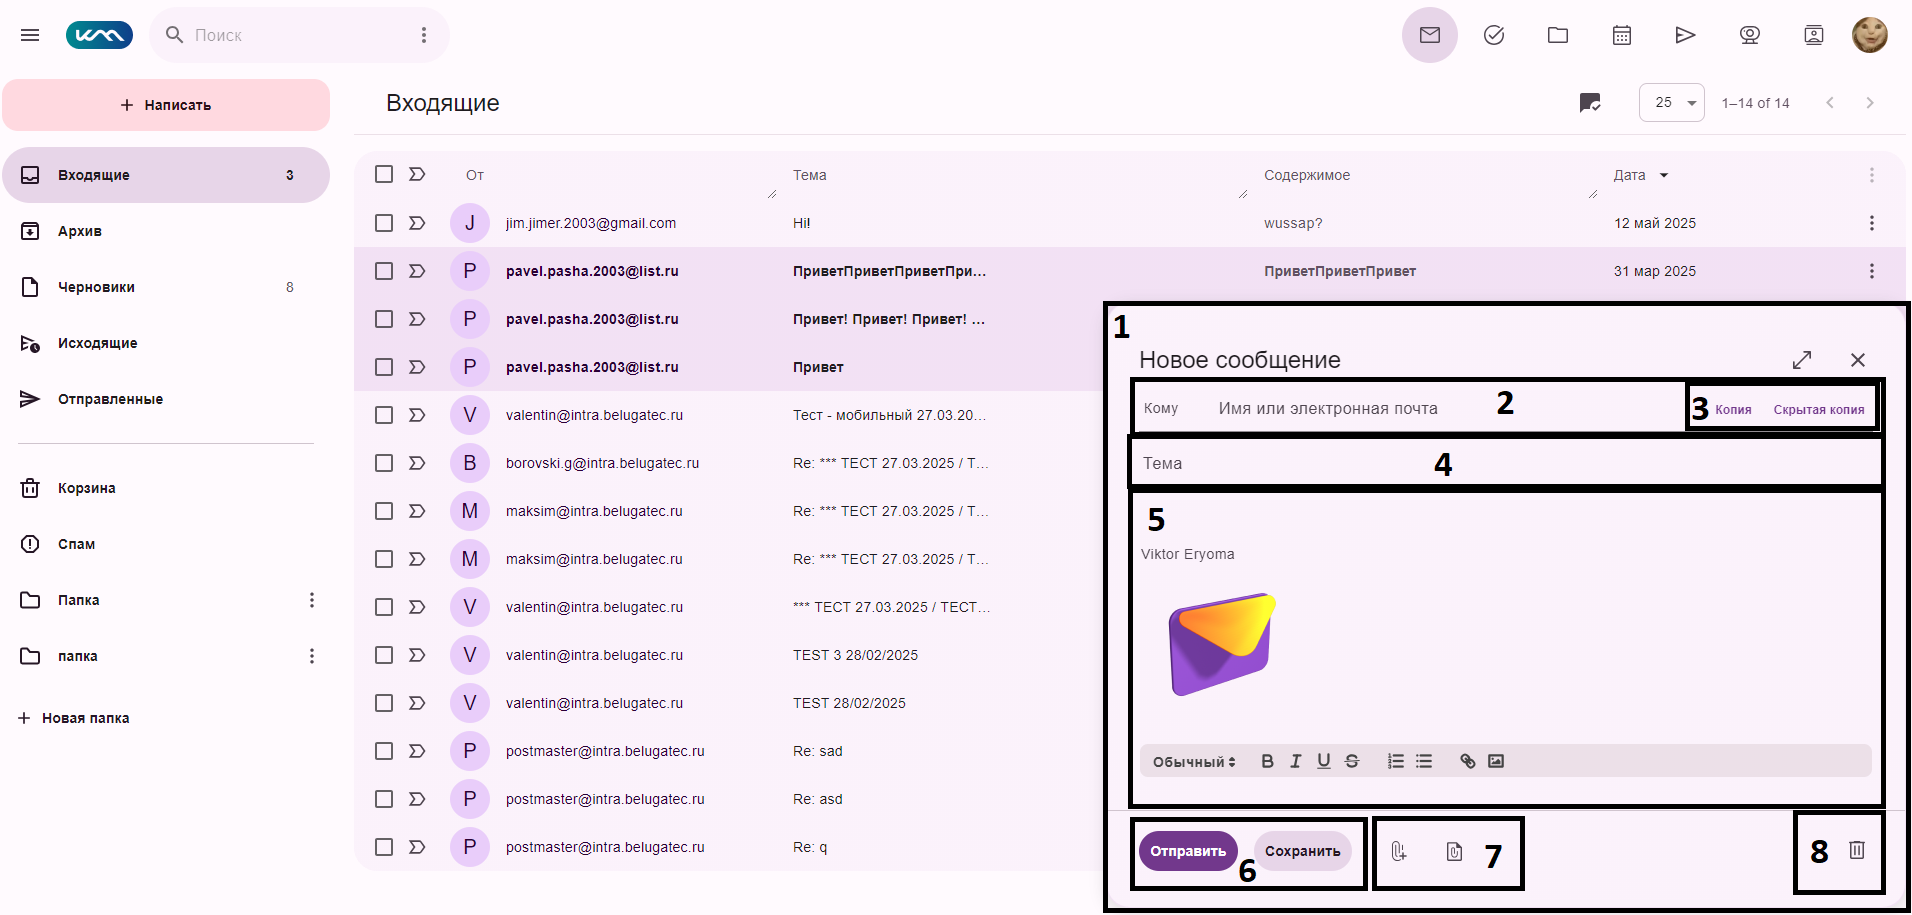
\includegraphics[width=1\linewidth]{images/почта2}
	\caption{Композиция интерфейса написания письма}
	\label{templ:image1b}
\end{figure}

Композиция интерфейса прикрепление файла из сервиса <<Файлы>> в сервисе <<Почта>> представлена на рисунке \ref{templ:image1c} и состоит из:
\begin{itemize}
  \item всплывающего окна(1);
  \item разделов с файлами (2);
  \item компонента файла с функцией выбора (3);
  \item кнопок для прикрепления файла (4);
\end{itemize}
\begin{figure}[H]
	\centering
	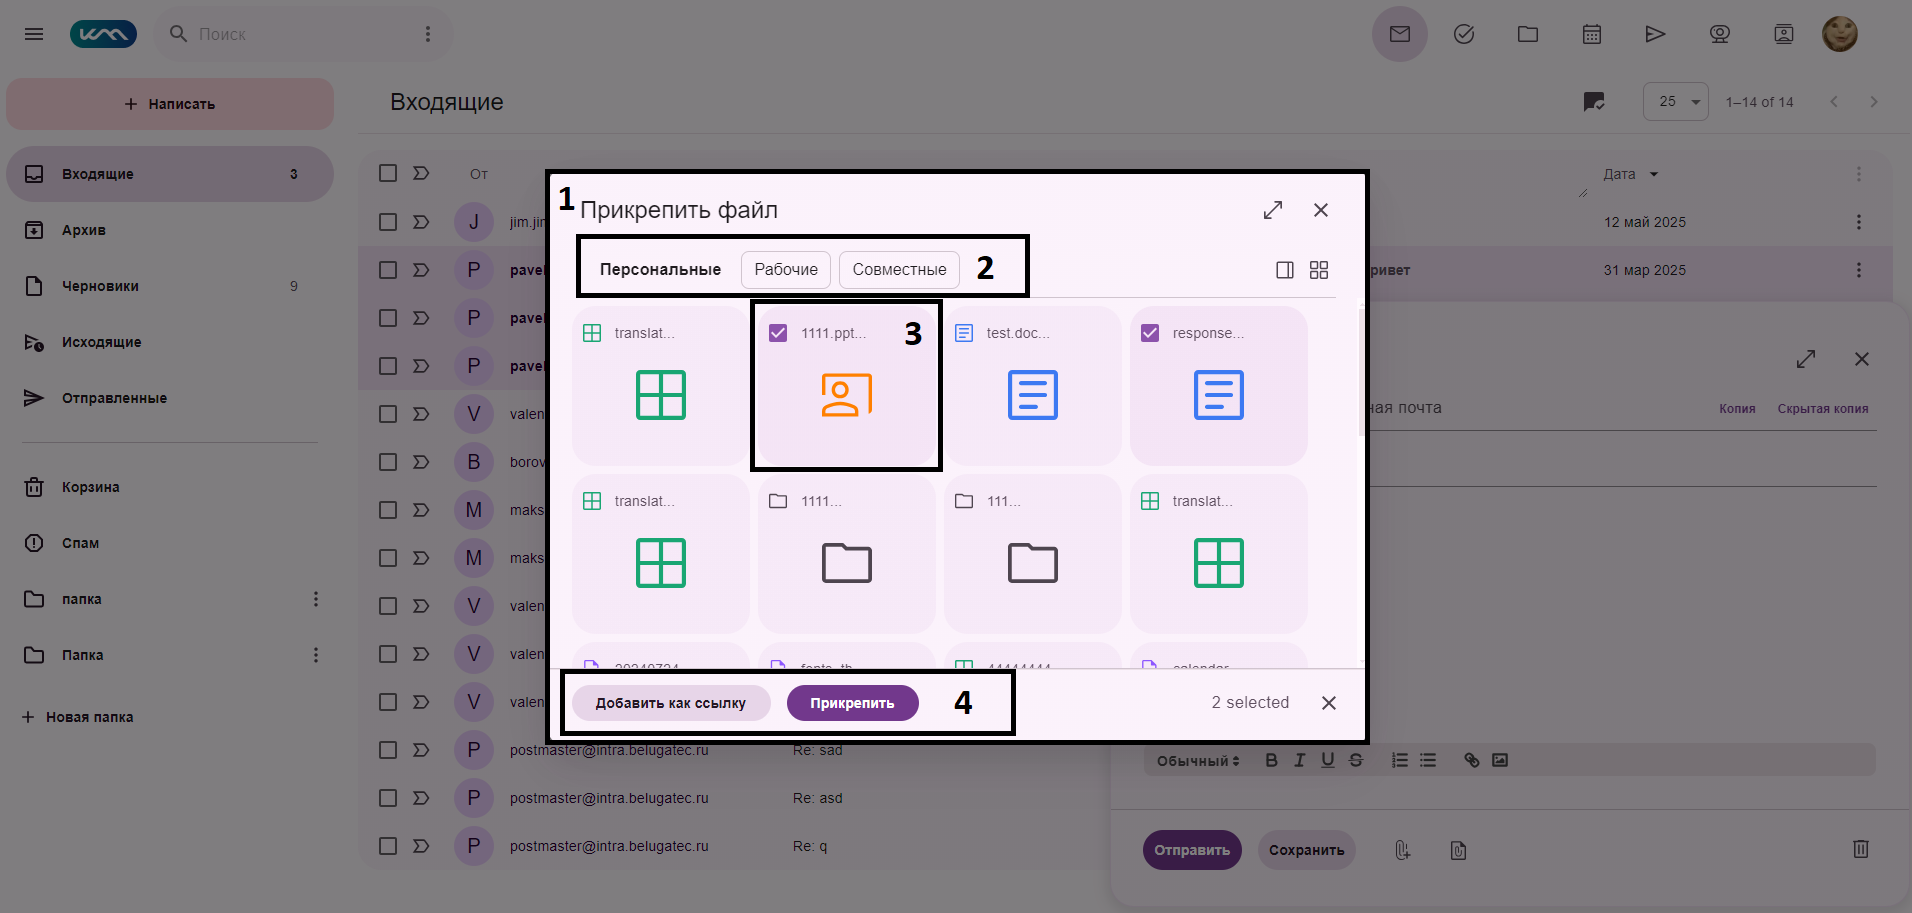
\includegraphics[width=1\linewidth]{images/почта3}
	\caption{Композиция интерфейса прикрепление файла}
	\label{templ:image1c}
\end{figure}

Композиция интерфейса создания папки в сервисе <<Почта>> представлена на рисунке \ref{templ:image1d} и состоит из:
\begin{itemize}
  \item всплывающего окна(1);
  \item поля ввода названия папки (2);
  \item кнопок действий (3);
\end{itemize}
\begin{figure}[H]
	\centering
	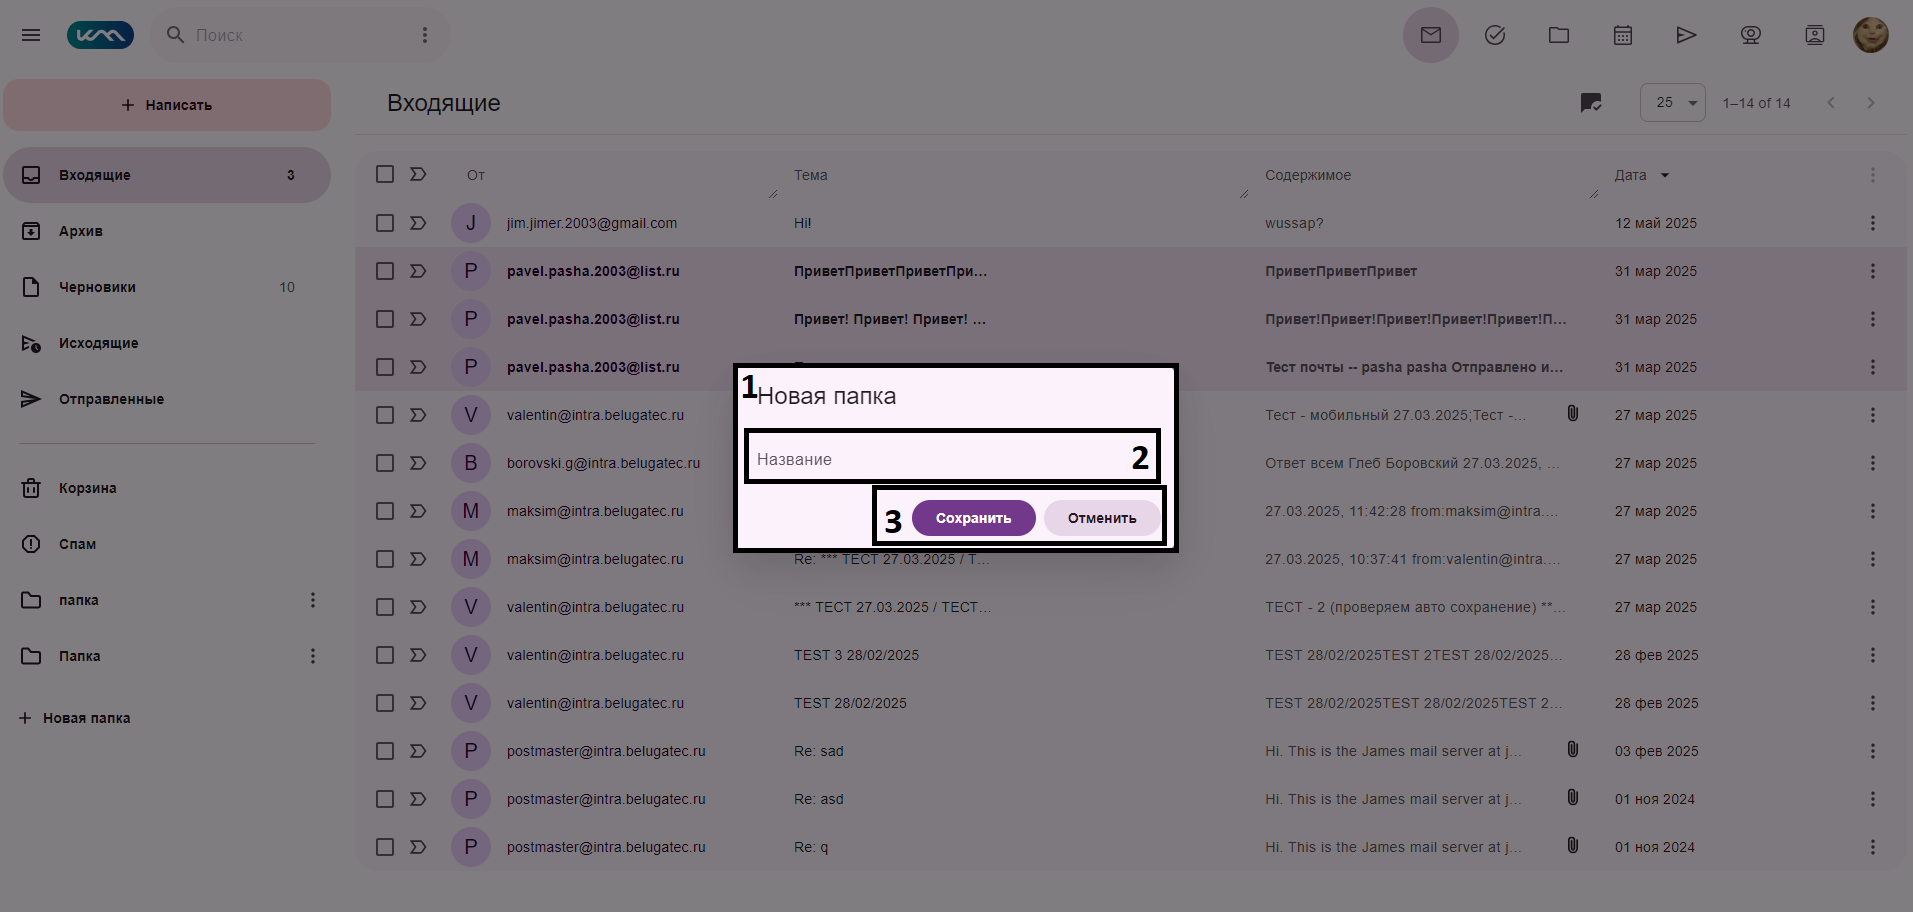
\includegraphics[width=1\linewidth]{images/почта4}
	\caption{Композиция интерфейса создания папки}
	\label{templ:image1d}
\end{figure}

Композиция интерфейса сервиса <<Видеоконференцсвязь>> представлена на рисунке \ref{templ:image2} и состоит из:
\begin{itemize}
  \item компонента навигации по сервисам (1);
  \item поля для ввода названия комнаты (2);
  \item кнопки для подключения к комнате (3);
  \item кнопки для подключения к запланированным встречам (4);
\end{itemize}
\begin{figure}[H]
	\centering
	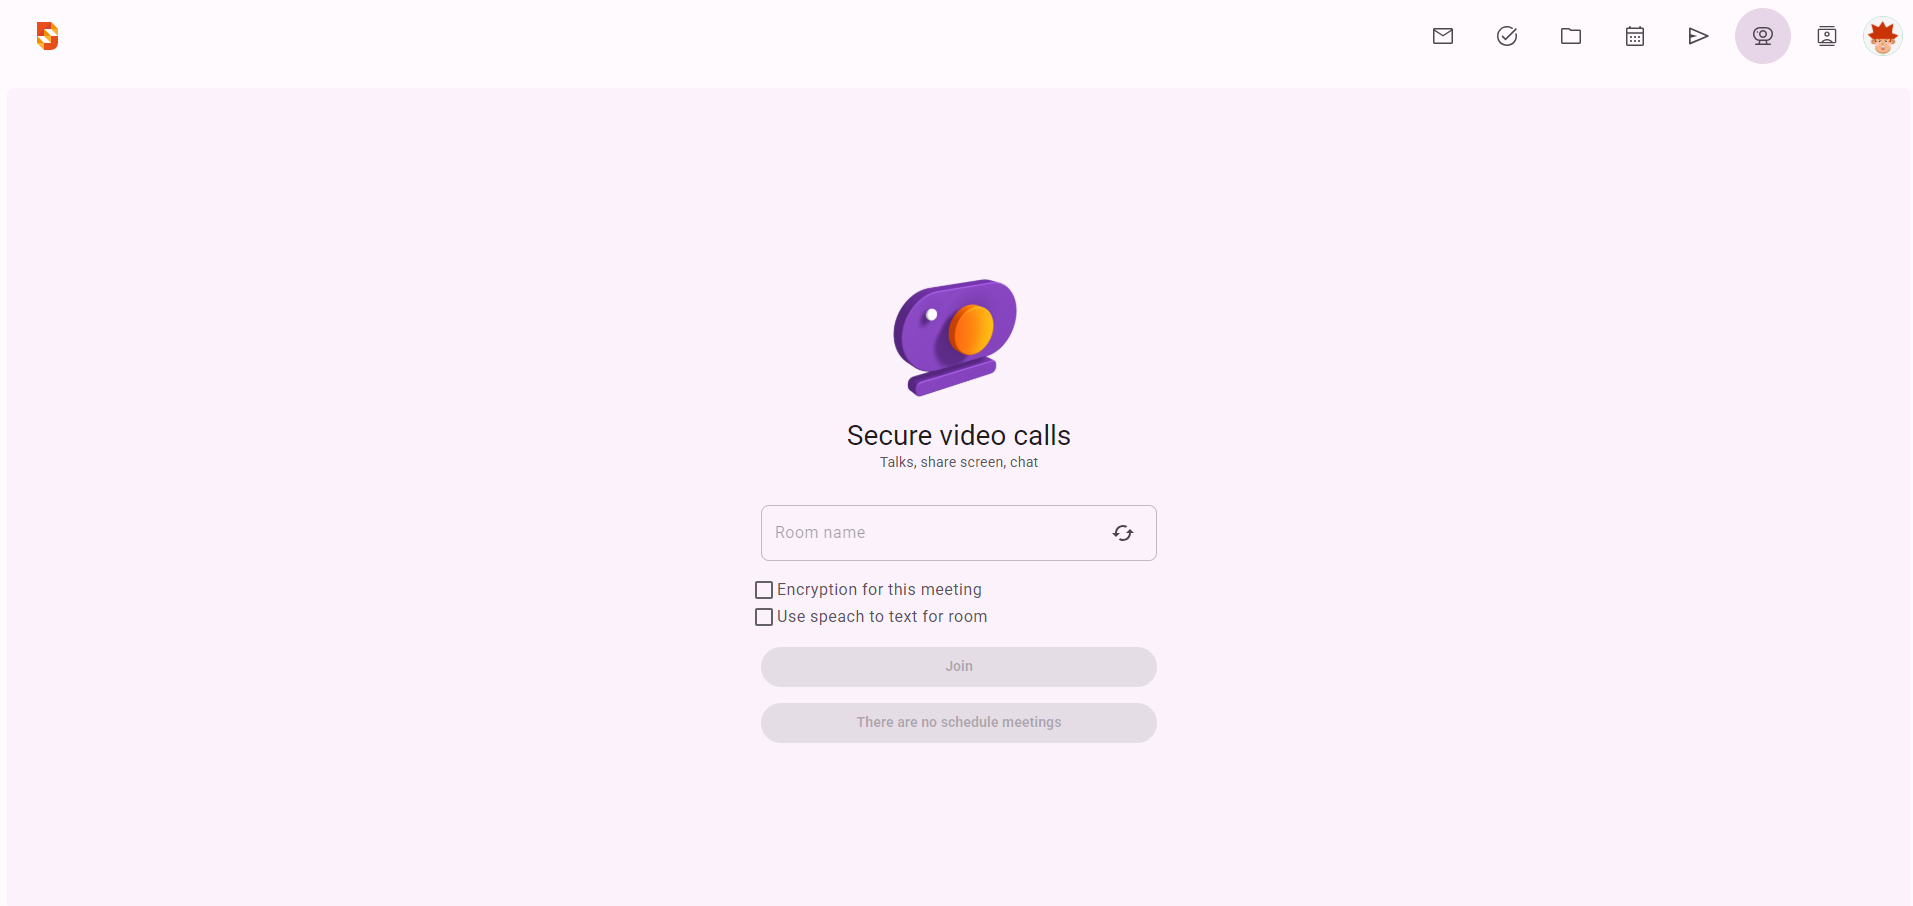
\includegraphics[width=1\linewidth]{images/вкс}
	\caption{Композиция интерфейса сервиса <<Видеоконференцсвязь>>}
	\label{templ:image2}
\end{figure}

Композиция интерфейса сервиса <<Календарь>> представлена на рисунке \ref{templ:image3} и состоит из:
\begin{itemize}
  \item компонента навигации по сервисам (1);
  \item кнопки для создания события (2);
  \item компонент уменьшенной версии календаря (3);
  \item кнопки фильтрации событий по типу (4);
  \item кнопки фильтрации событий по дате (5);
  \item окно для основной работы с календарём (6);
\end{itemize}
\begin{figure}[H]
	\centering
	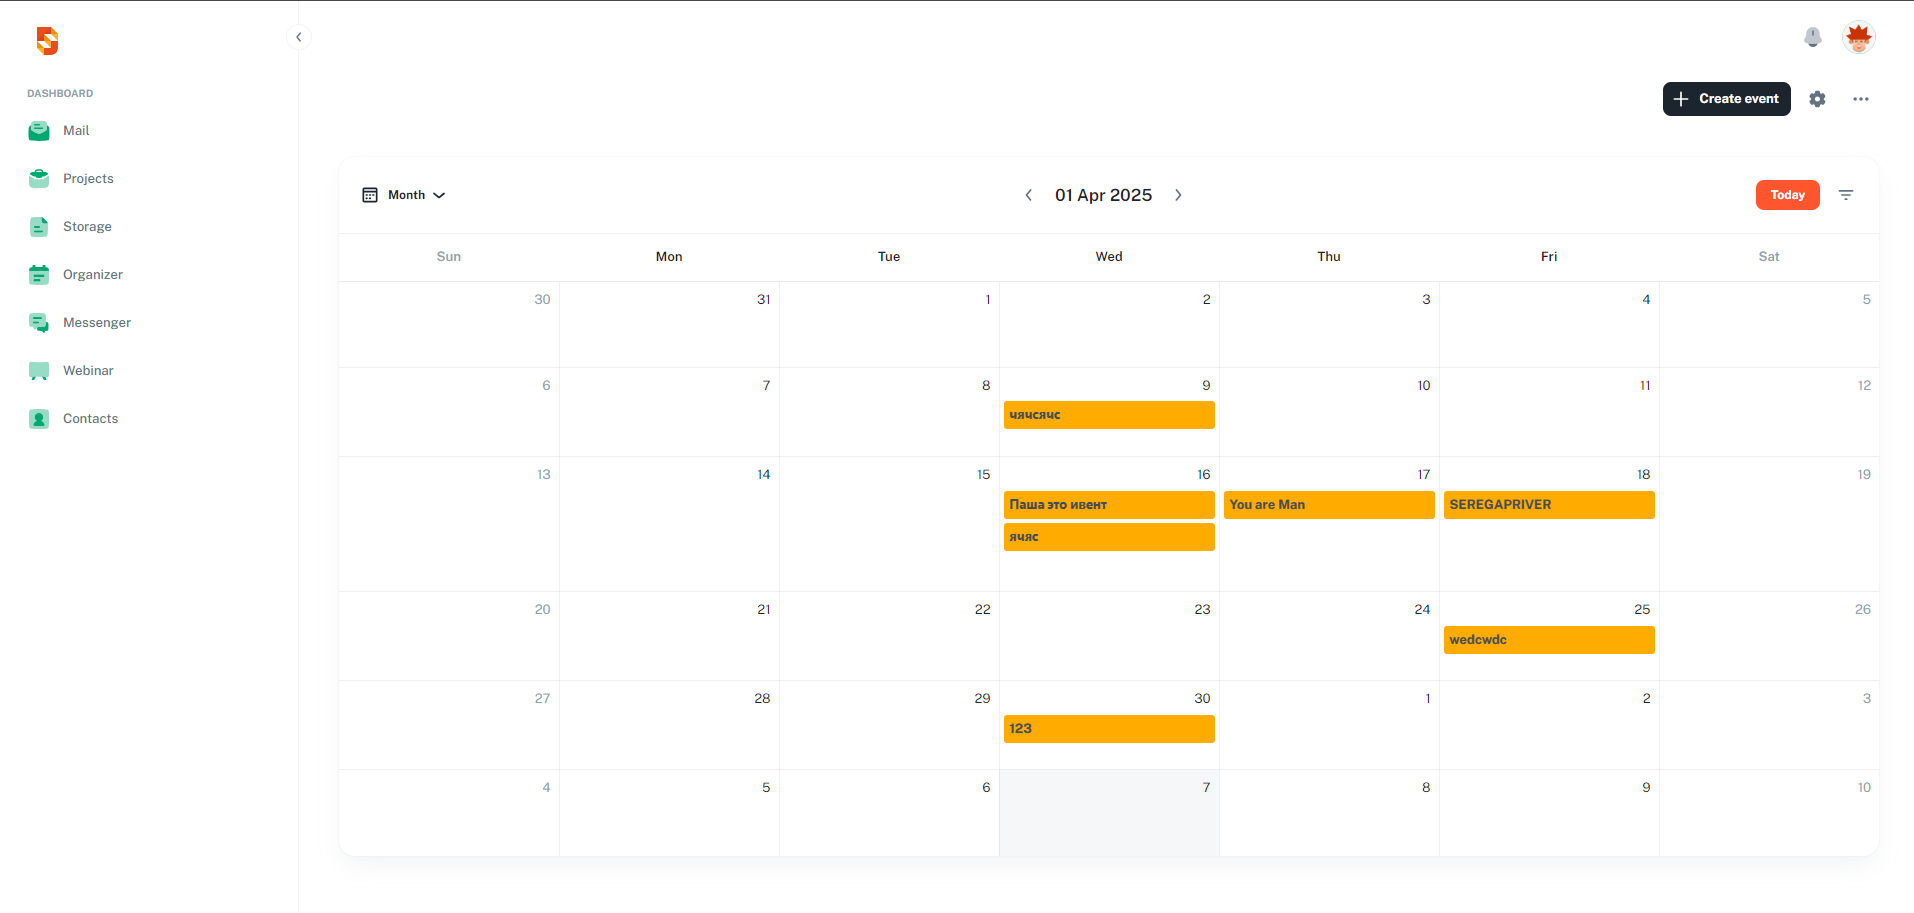
\includegraphics[width=1\linewidth]{images/календарь}
	\caption{Композиция интерфейса сервиса <<Календарь>>}
	\label{templ:image3}
\end{figure}

Композиция интерфейса создания события в сервисе <<Календарь>> представлена на рисунке \ref{templ:image3b} и состоит из:
\begin{itemize}
  \item всплывающего окна (1);
  \item кнопки для выбора категории (2);
  \item поля для ввода названия события (3);
  \item поля для ввода описания события (4);
  \item поля для ввода даты начала события и его параметров (5);
  \item поля для ввода названия видеоконференции (6);
  \item поля для выбора участников из сервиса <<Контакты>> (7);
\end{itemize}
\begin{figure}[H]
	\centering
	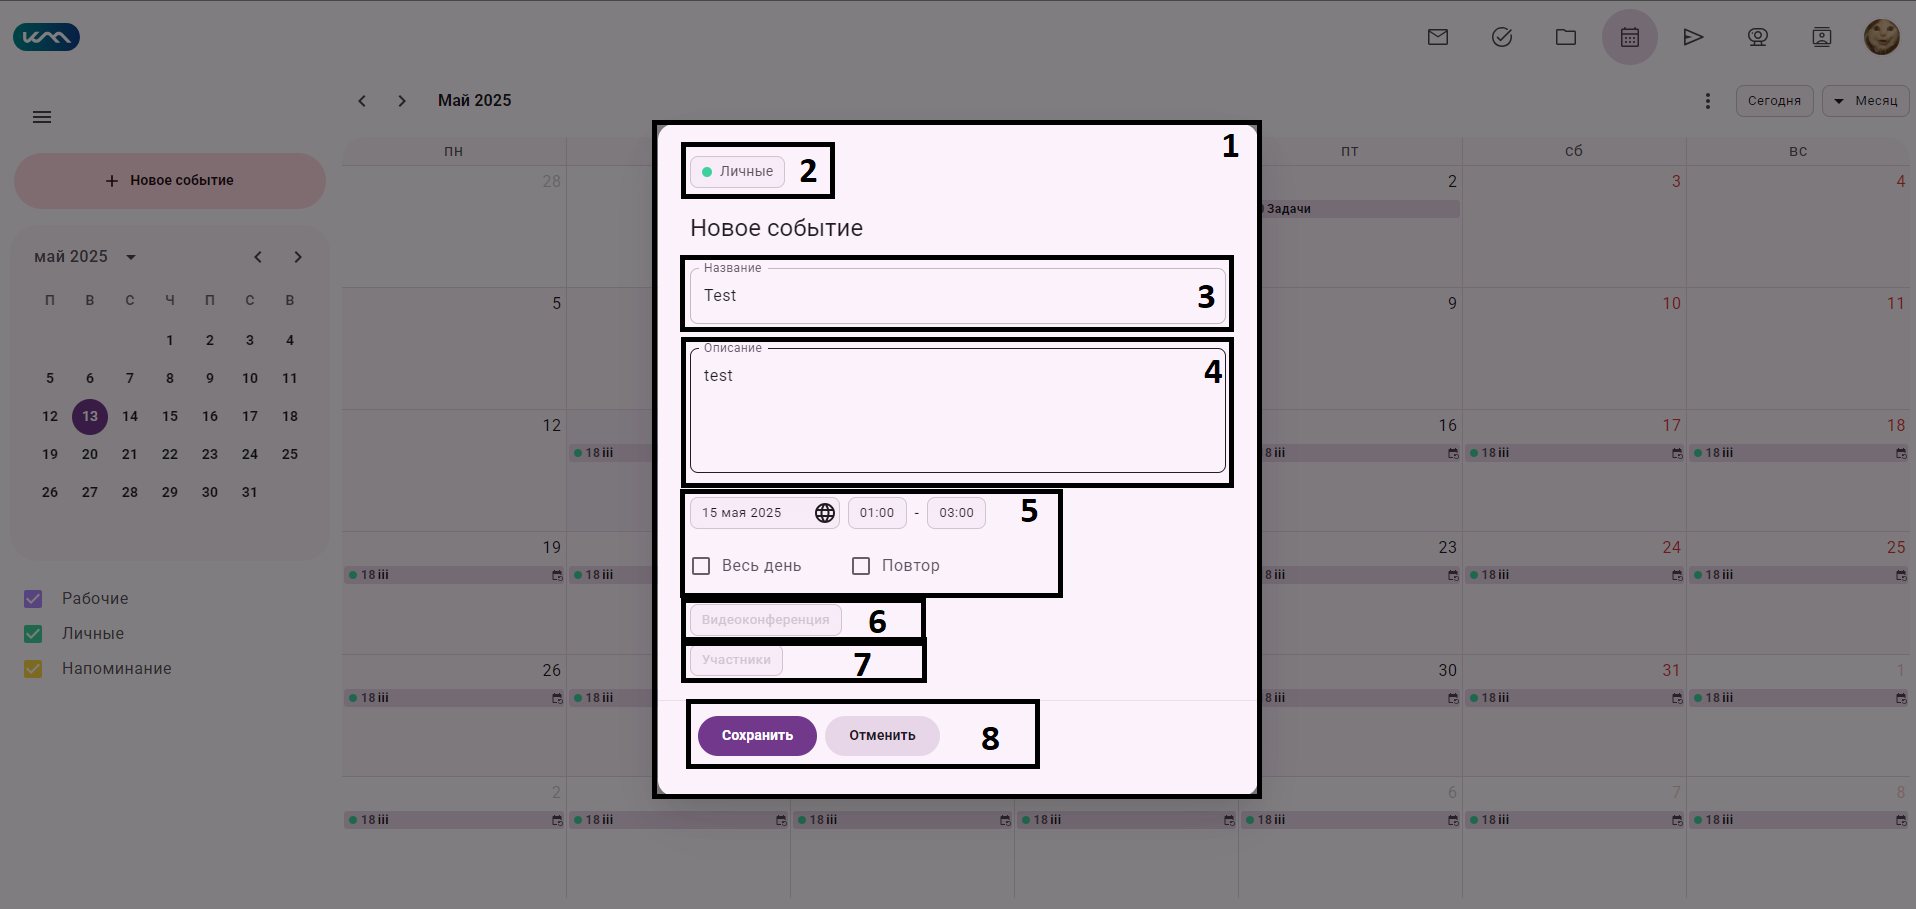
\includegraphics[width=1\linewidth]{images/календарь2}
	\caption{Композиция интерфейса создания события}
	\label{templ:image3b}
\end{figure}

Композиция интерфейса просмотра события в сервисе <<Календарь>> представлена на рисунке \ref{templ:image3c} и состоит из:
\begin{itemize}
  \item всплывающего окна (1);
  \item кнопок для редактирования, создания ссылки, удаления события (2);
  \item раздела с подробной информацией о событии (3);
  \item кнопок для подключения к ВКС, копирования события, прикрепления файла из сервиса <<Файлы>> (4);
  \item раздела с подробной информацией об участниках (5);
\end{itemize}
\begin{figure}[H]
	\centering
	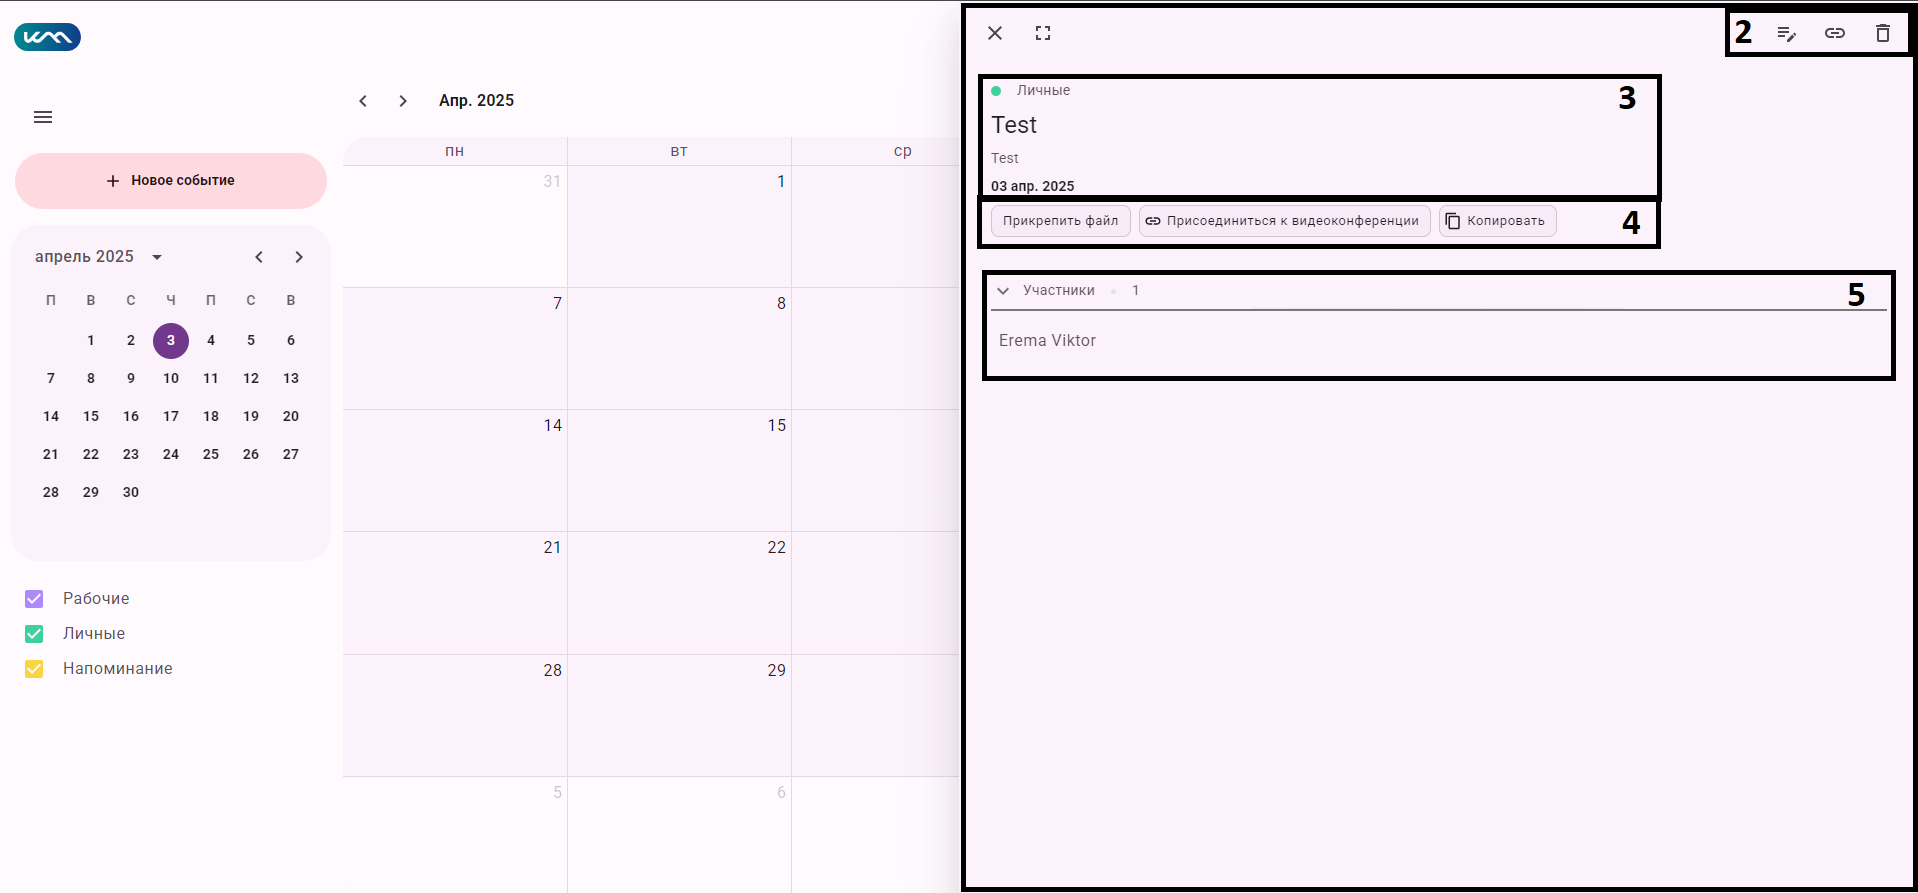
\includegraphics[width=1\linewidth]{images/календарь3}
	\caption{Композиция интерфейса просмотра события}
	\label{templ:image3c}
\end{figure}

Композиция интерфейса сервиса <<Панель управления>> представлена на рисунке \ref{templ:image4} и состоит из:
\begin{itemize}
  \item компонента навигации по сервисам (1);
  \item компонента "виджета" сервиса <<Почта>> (2);
  \item компонента "виджета" сервиса <<Проекты>> (3);
  \item компонента "виджета" сервиса <<Файлы>> (4);
  \item компонента "виджета" сервиса <<Календарь>> (5);
  \item компонента "виджета" сервиса <<Разговоры>> (6);
  \item компонента "виджета" сервиса <<Видеоконференцсвязь>> (7);
  \item компонента "виджета" сервиса <<Контакты>> (8);
\end{itemize}
\begin{figure}[H]
	\centering
	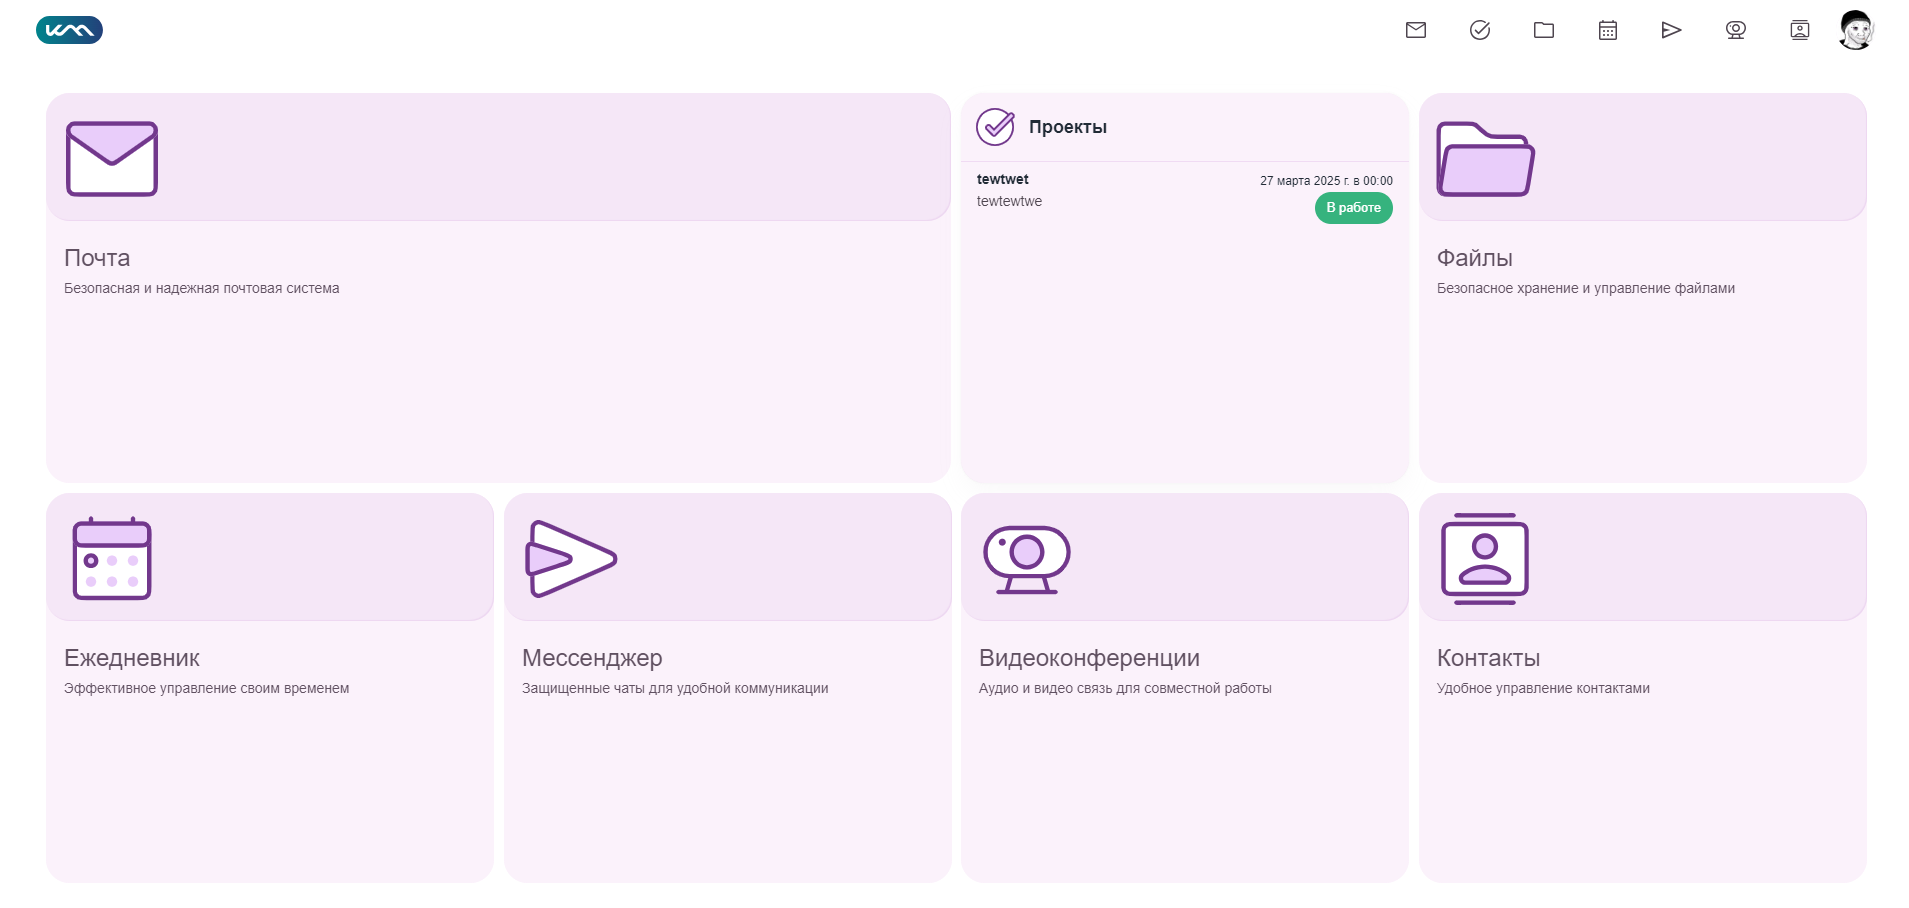
\includegraphics[width=1\linewidth]{images/дашборд}
	\caption{Композиция интерфейса сервиса <<Панель управления>>}
	\label{templ:image4}
\end{figure}

Композиция интерфейса сервиса <<Контакты>> представлена на рисунке \ref{templ:image5} и состоит из:
\begin{itemize}
  \item компонента навигации по сервисам (1);
  \item кнопки для создания контакта (2);
  \item списка папок (3);
  \item окна для работы с контактами (4);
  \item компонента пагинации (5);
\end{itemize}
\begin{figure}[H]
	\centering
	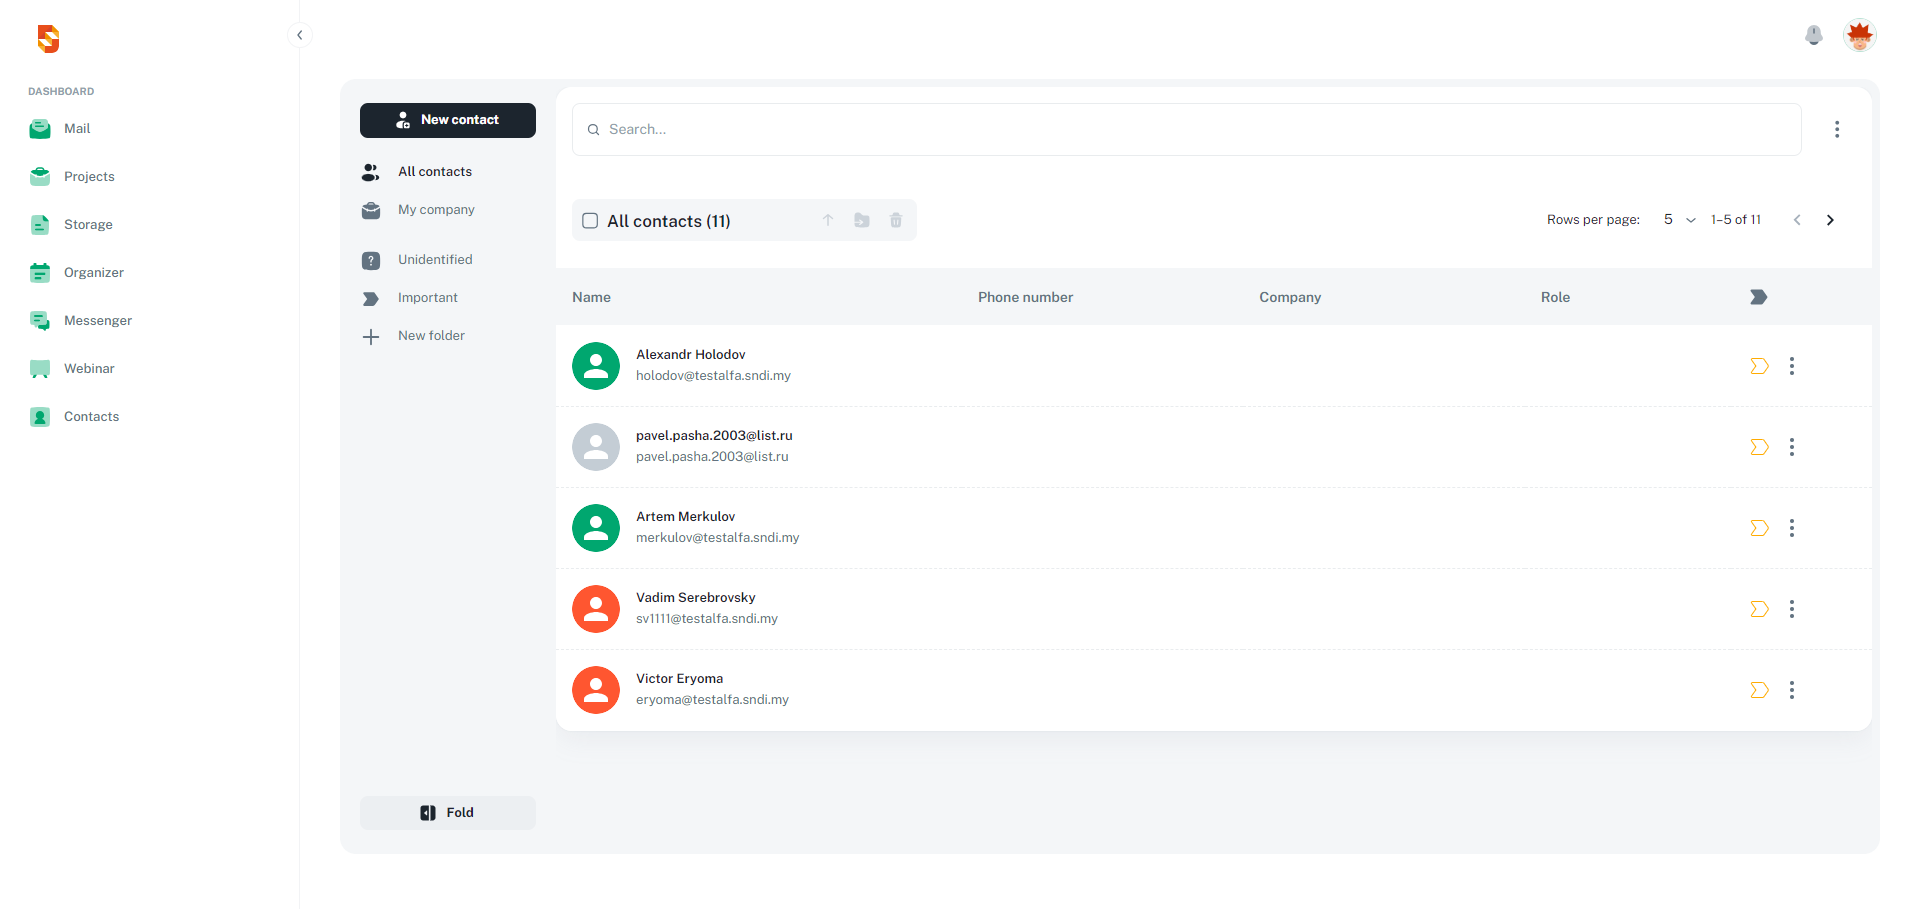
\includegraphics[width=1\linewidth]{images/контакты}
	\caption{Композиция интерфейса сервиса <<Контакты>>}
	\label{templ:image5}
\end{figure}

Композиция интерфейса создания контакта в сервисе <<Контакты>> представлена на рисунке \ref{templ:image5b} и состоит из:
\begin{itemize}
  \item всплывающего окна (1);
  \item поля для ввода имени (2);
  \item поля для ввода фамилии (3);
  \item поля для ввода даты рождения (4);
  \item поля для ввода компании (5);
  \item поля для ввода должности (6);
  \item поля для ввода почты (7);
  \item поля для ввода телефона (8);
  \item кнопок действий (9);
\end{itemize}
\begin{figure}[H]
	\centering
	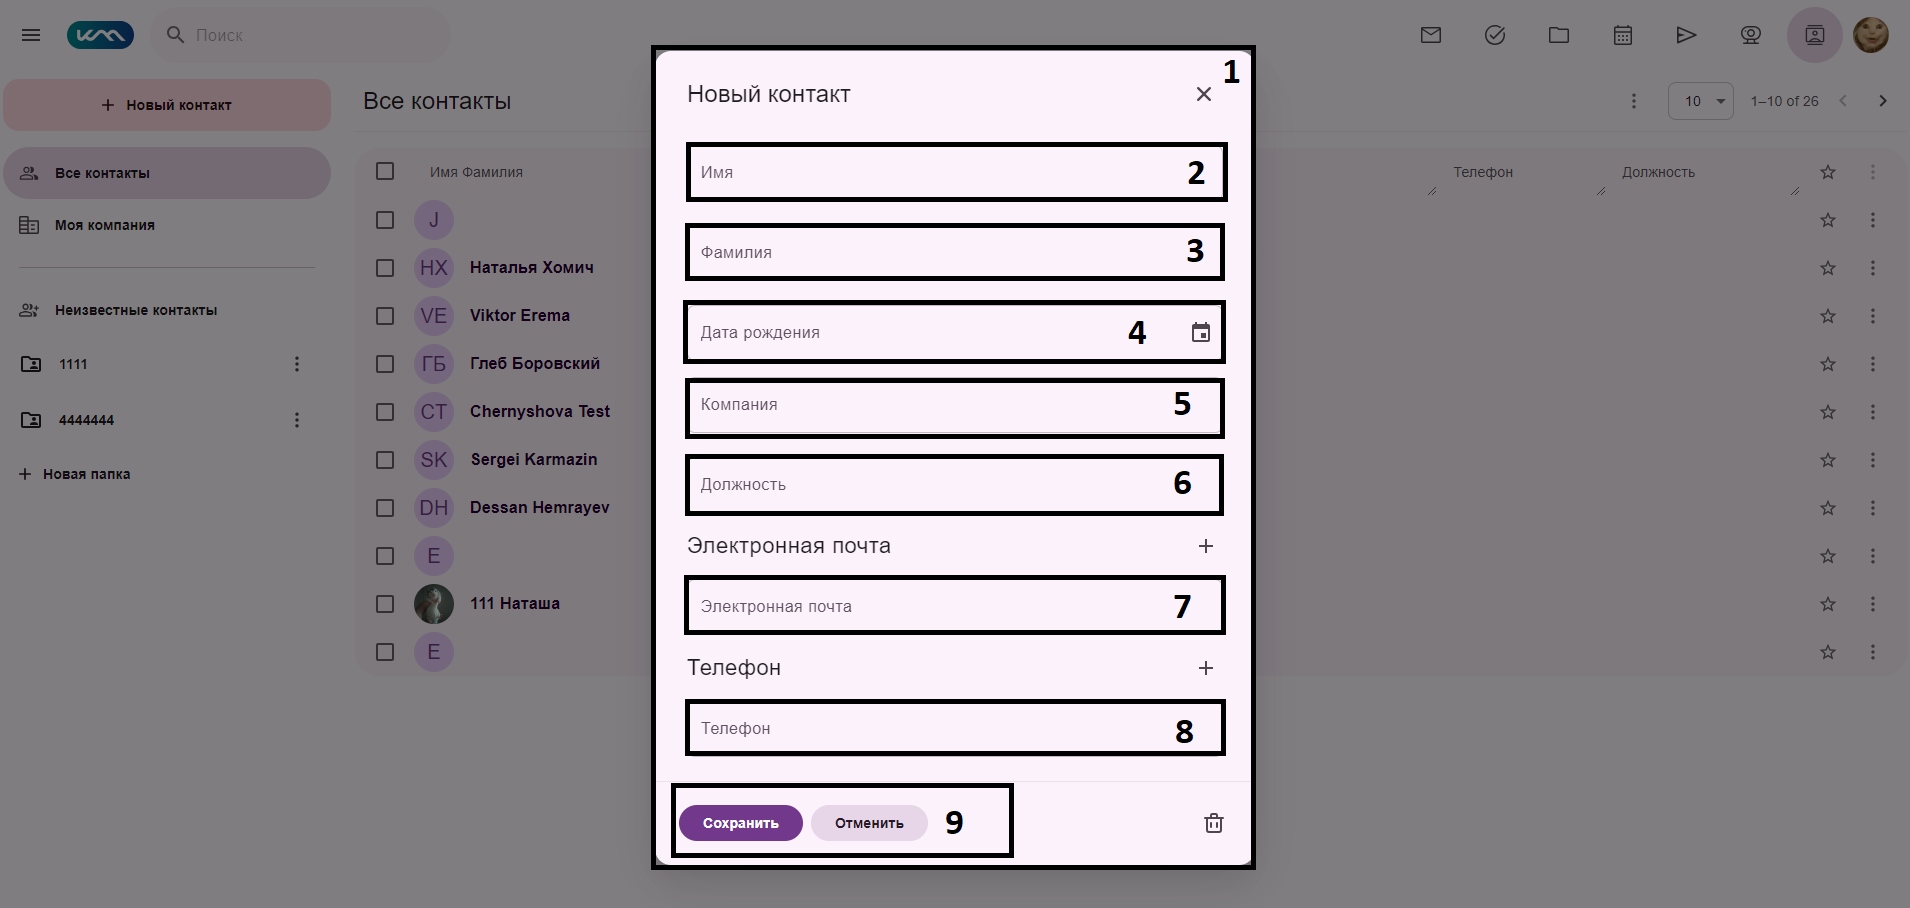
\includegraphics[width=1\linewidth]{images/контакты2}
	\caption{Композиция интерфейса создания контакта}
	\label{templ:image5b}
\end{figure}

Композиция интерфейса просмотра контакта в сервисе <<Контакты>> представлена на рисунке \ref{templ:image5b} и состоит из:
\begin{itemize}
  \item окна с информацией о контакте (1);
  \item кнопок для скачивания, редактирования, удаления и отправки контакта (2);
  \item кнопки для написания письма этому человеку в сервисе <<Почта>> (3);
  \item окна с подробной информацией о контакте (4);
\end{itemize}
\begin{figure}[H]
	\centering
	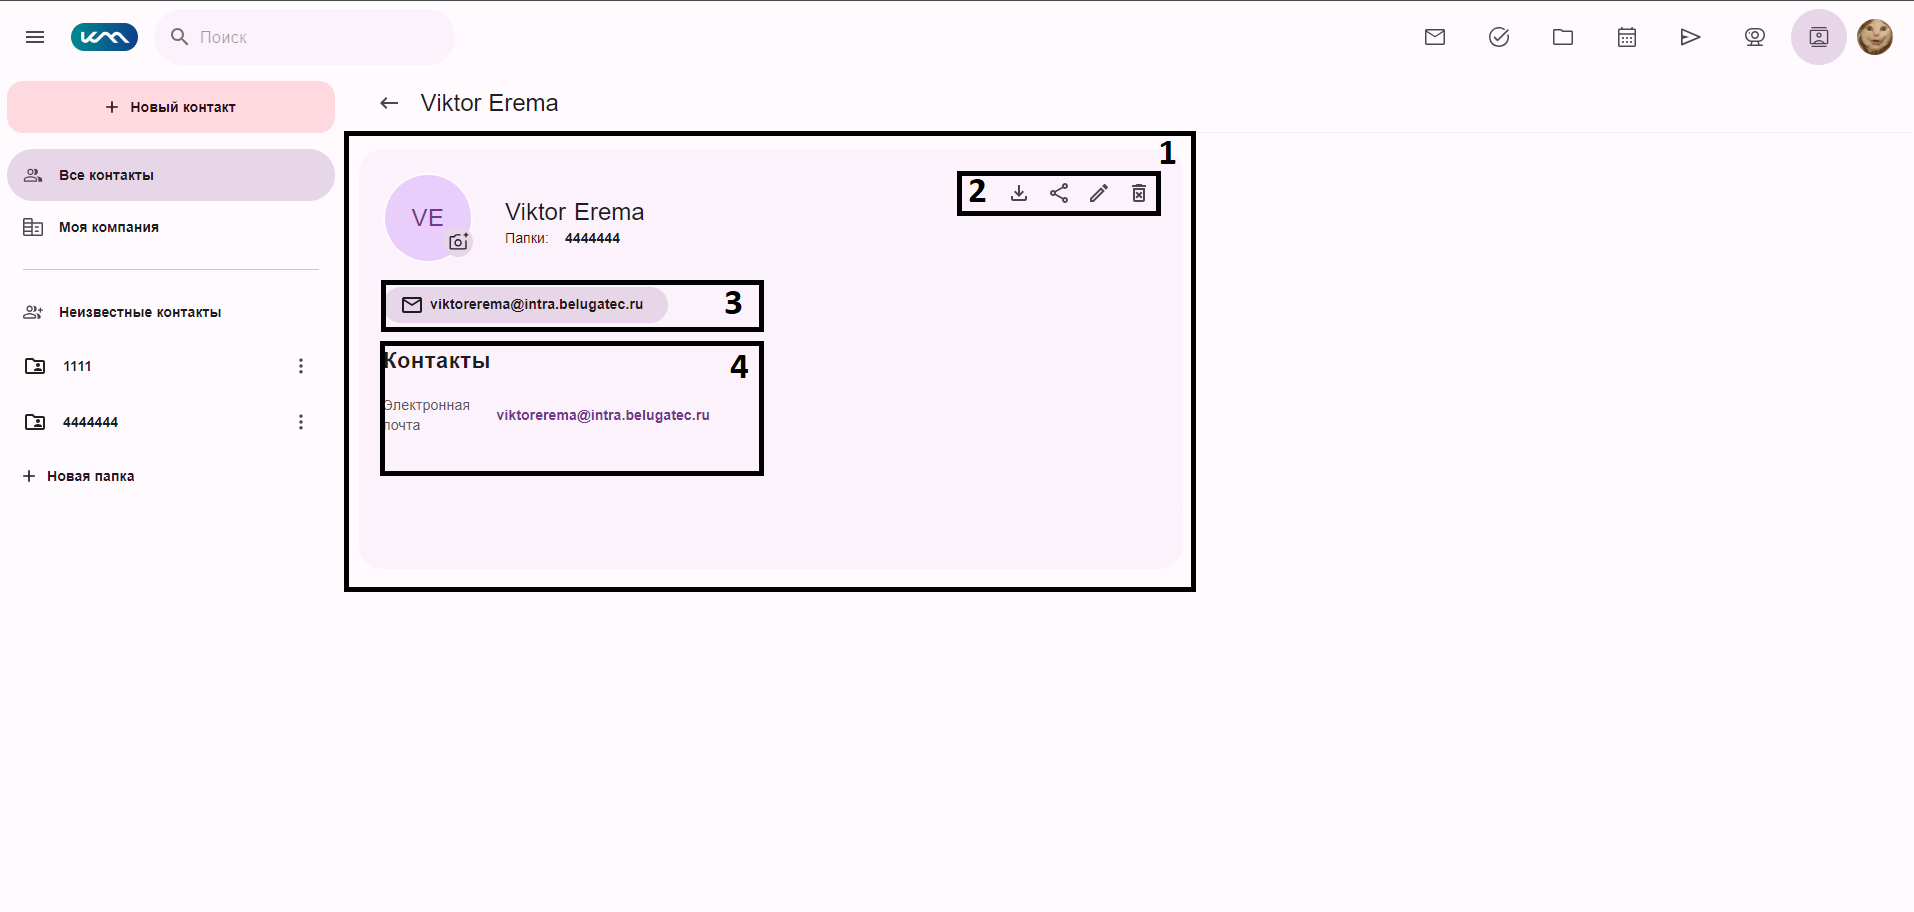
\includegraphics[width=1\linewidth]{images/контакты3}
	\caption{Композиция интерфейса просмотра контакта}
	\label{templ:image5b}
\end{figure}

Композиция интерфейса создания папки в сервисе <<Контакты>> представлена на рисунке \ref{templ:image5c} и состоит из:
\begin{itemize}
  \item всплывающего окна (1);
  \item поля для ввода названия папки (2);
  \item кнопок действий (3);
\end{itemize}
\begin{figure}[H]
	\centering
	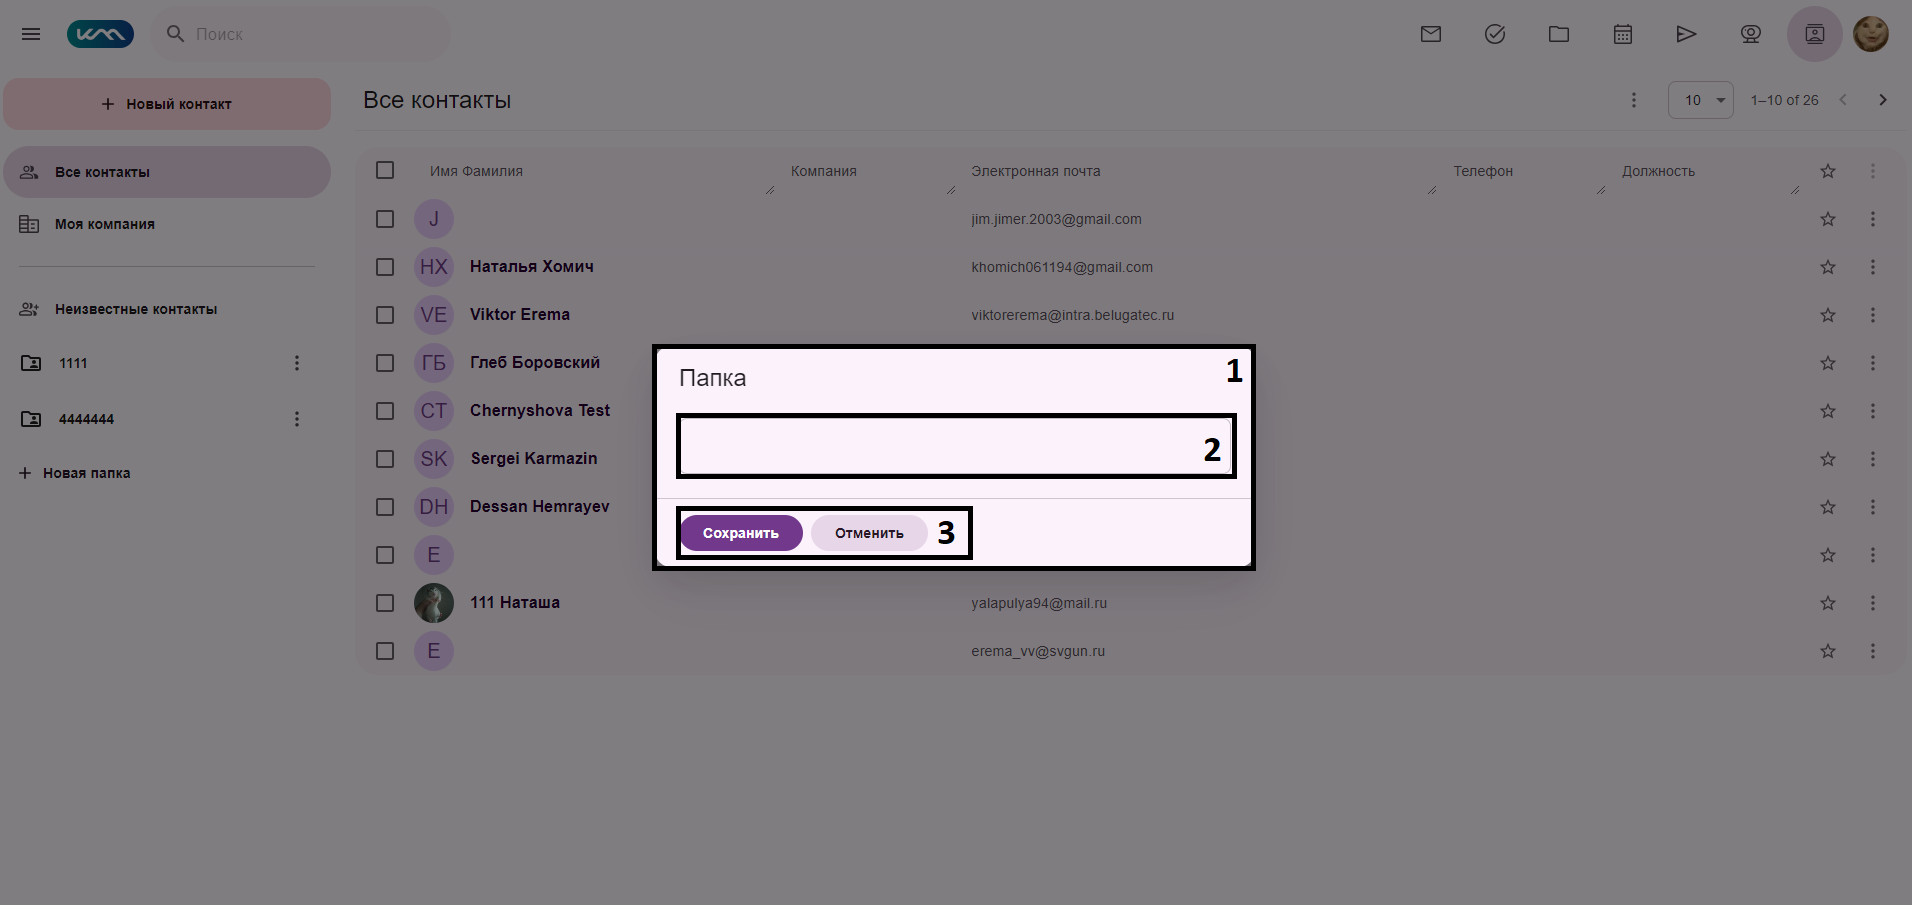
\includegraphics[width=1\linewidth]{images/контакты4}
	\caption{Композиция интерфейса создания папки}
	\label{templ:image5c}
\end{figure}

Композиция интерфейса сервиса <<Настройки>> представлена на рисунке \ref{templ:image6} и состоит из:
\begin{itemize}
  \item компонента навигации по сервисам (1);
  \item компонента навигации по разделам (2);
  \item кнопки для выхода из учётной записи (3);
  \item раздела смены темы (4);
  \item раздела смены цветовой палитры (5);
  \item раздела редактирования подписи электронной почты (6);
\end{itemize}
\begin{figure}[H]
	\centering
	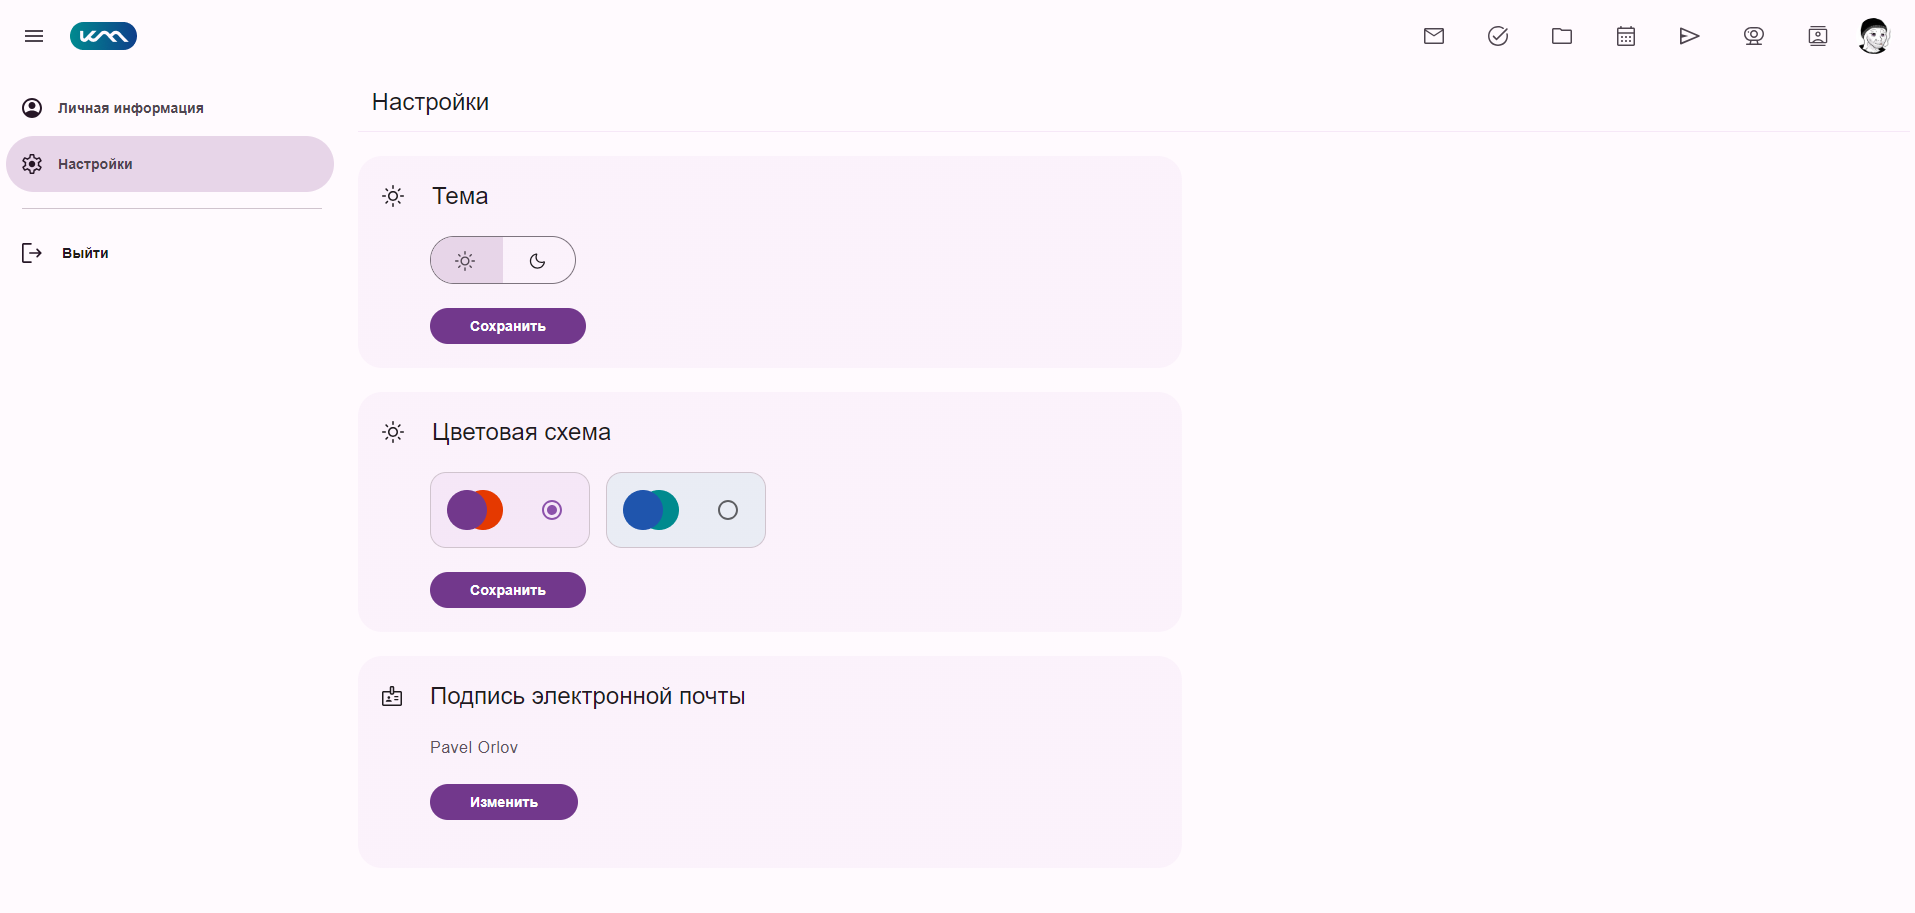
\includegraphics[width=1\linewidth]{images/настройки}
	\caption{Композиция интерфейса сервиса <<Настройки>>}
	\label{templ:image6}
\end{figure}

Композиция интерфейса изменения цифровой подписи в сервисе <<Настройки>> представлена на рисунке \ref{templ:image6b} и состоит из:
\begin{itemize}
  \item всплывающего окна (1);
  \item поля для ввода цифровой подписи (2);
  \item кнопок действий (3);
\end{itemize}
\begin{figure}[H]
	\centering
	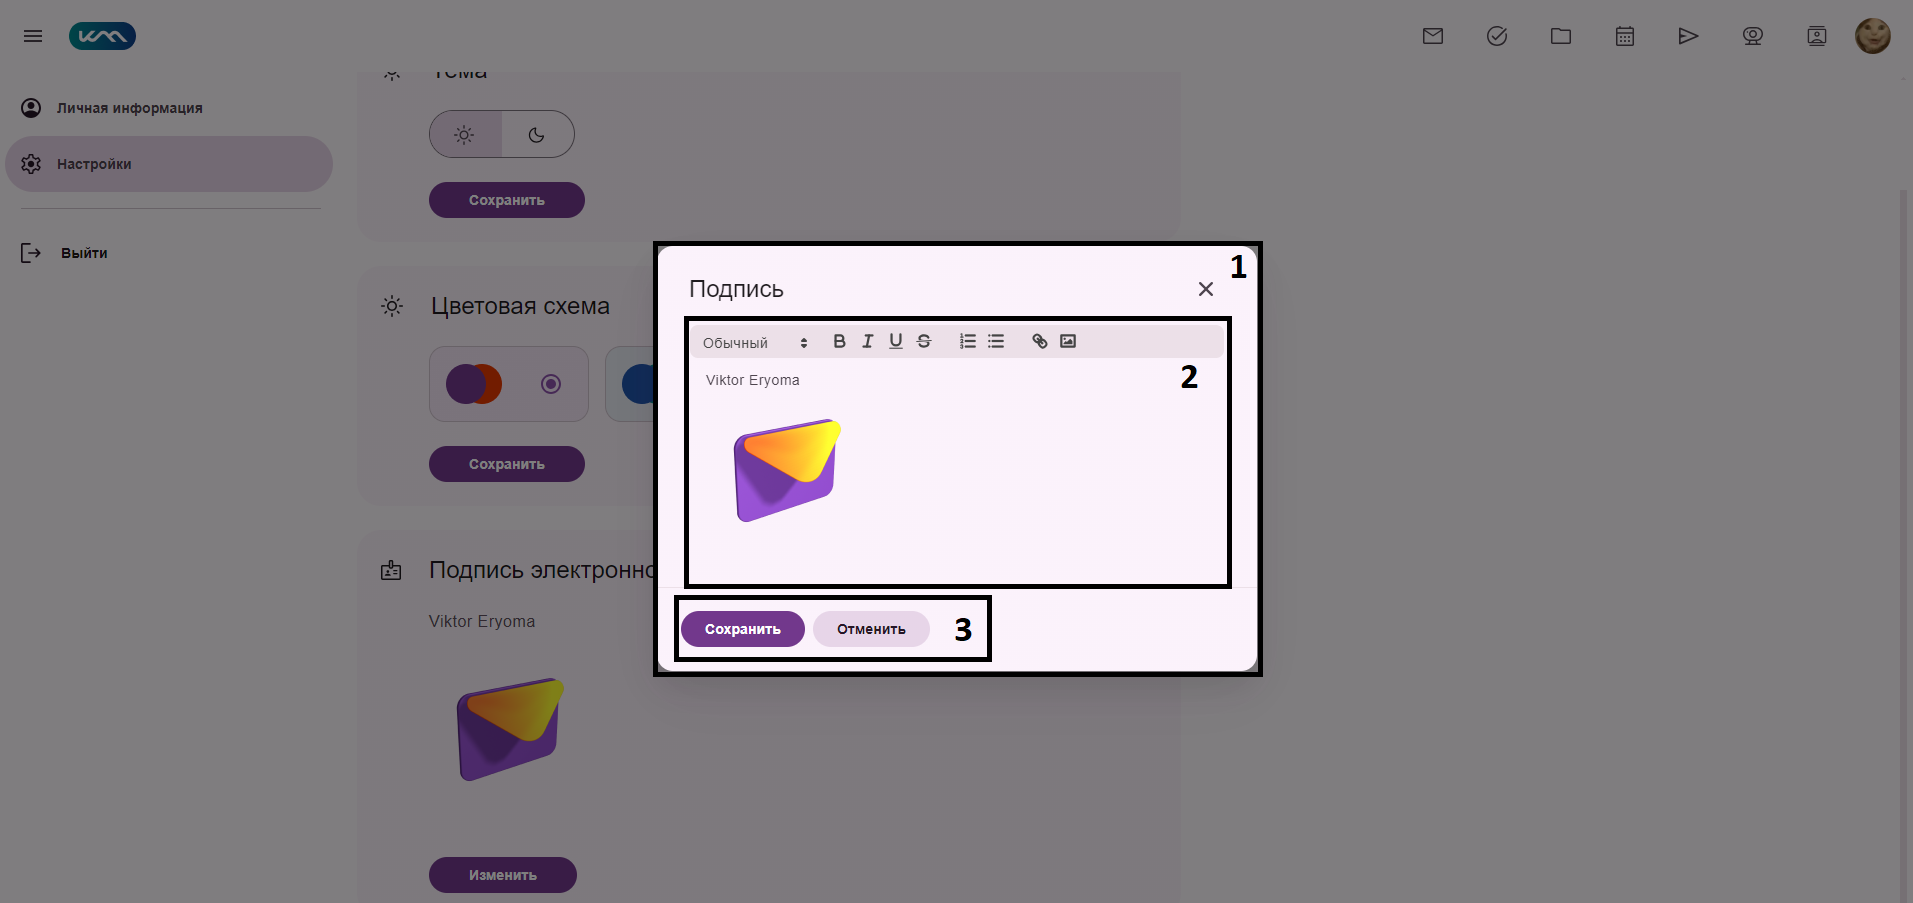
\includegraphics[width=1\linewidth]{images/настройки2}
	\caption{Композиция интерфейса изменения цифровой подписи}
	\label{templ:image6b}
\end{figure}

Композиция интерфейса сервиса <<Проекты>> представлена на рисунке \ref{templ:image7} и состоит из:
\begin{itemize}
  \item компонента навигации по сервисам (1);
  \item кнопки для создания раздела (2);
  \item компонента навигации по разделам (3);
  \item окна для работы с задачами (4);
  \item кнопки для создания задачи (5);
\end{itemize}
\begin{figure}[H]
	\centering
	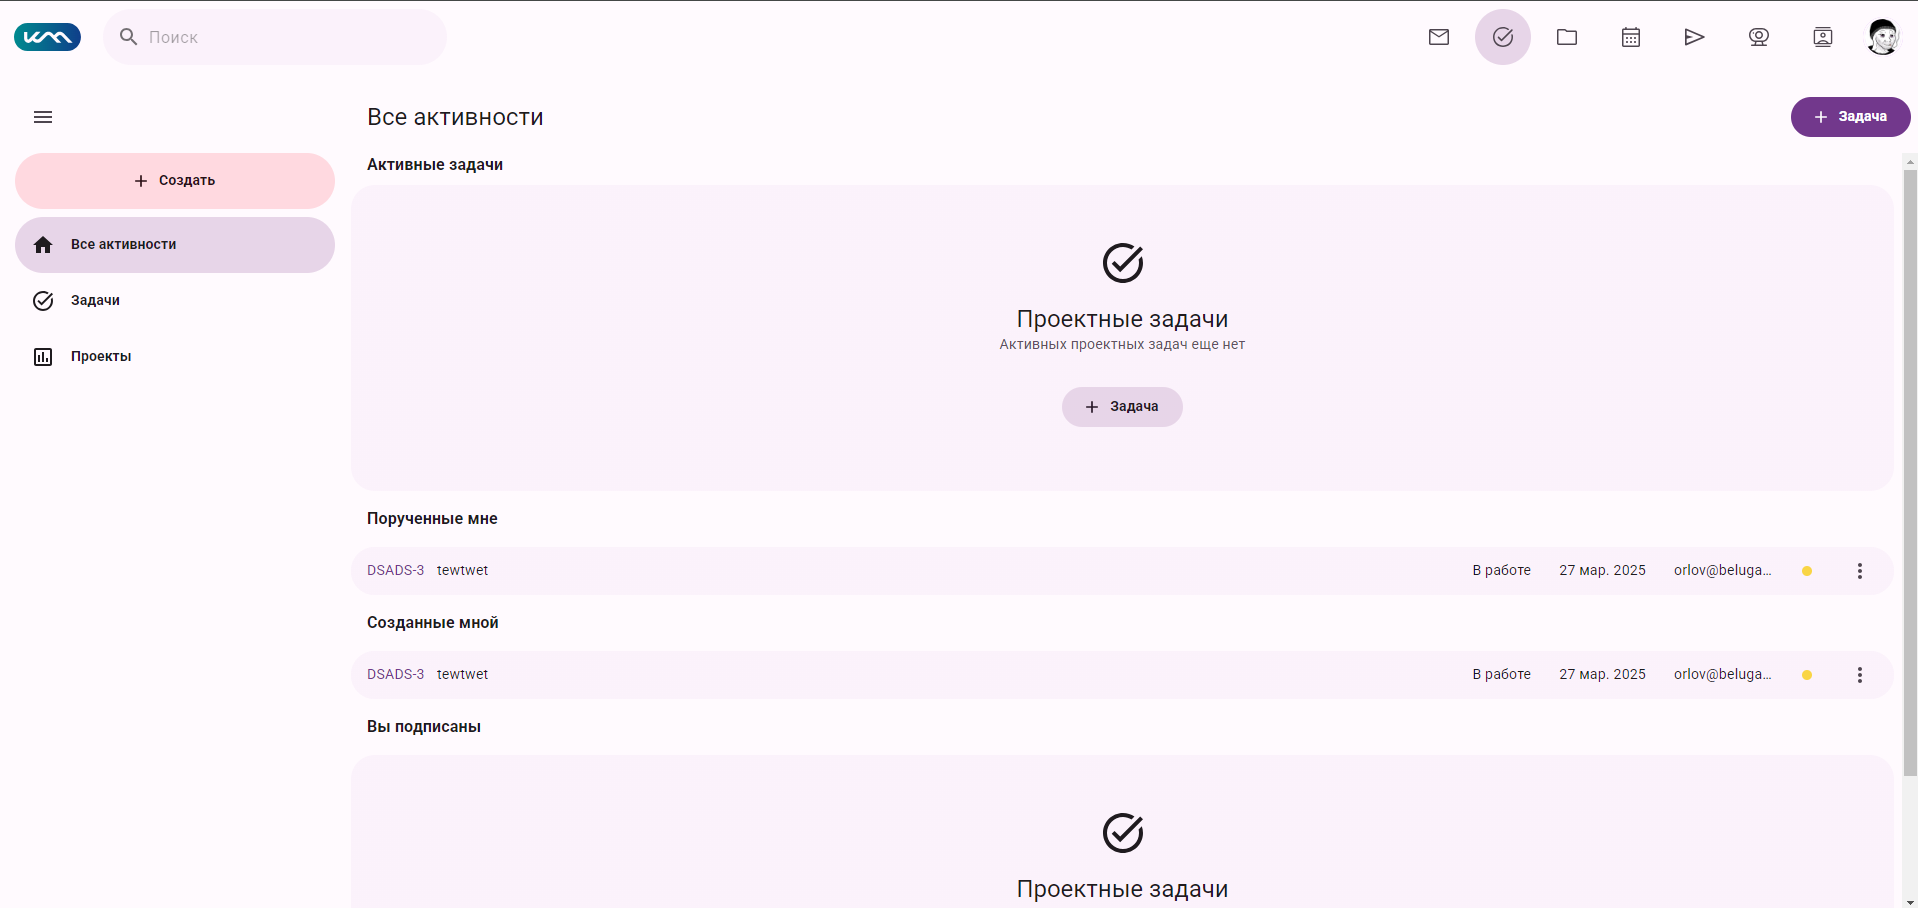
\includegraphics[width=1\linewidth]{images/проекты}
	\caption{Композиция интерфейса сервиса <<Проекты>>}
	\label{templ:image7}
\end{figure}

Композиция интерфейса создания проекта в сервисе <<Проекты>> представлена на рисунке \ref{templ:image7b} и состоит из:
\begin{itemize}
  \item всплывающего окна (1);
  \item поля для ввода названия проекта (2);
  \item поля для ввода описания проекта (3);
  \item кнопок действий (4);
\end{itemize}
\begin{figure}[H]
	\centering
	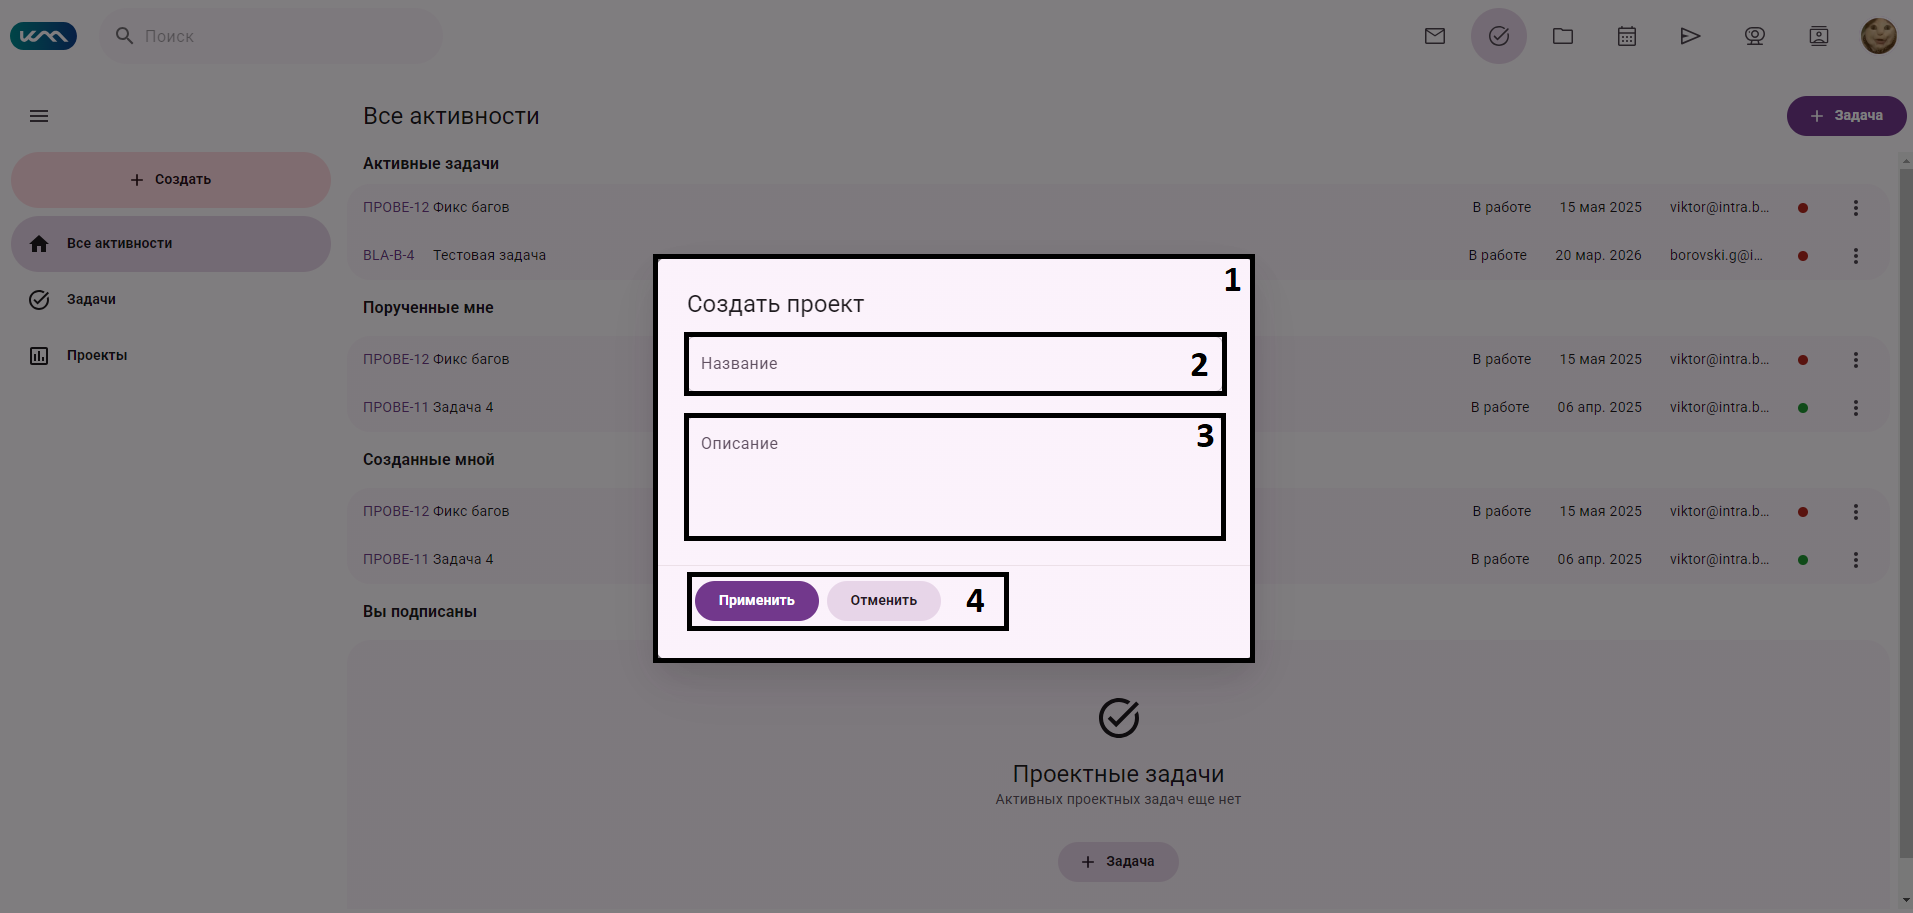
\includegraphics[width=1\linewidth]{images/проекты2}
	\caption{Композиция интерфейса создания проекта}
	\label{templ:image7b}
\end{figure}

Композиция интерфейса создания задачи в сервисе <<Проекты>> представлена на рисунке \ref{templ:image7c} и состоит из:
\begin{itemize}
  \item всплывающего окна (1);
  \item кнопки для выбора проекта (2);
  \item поля для ввода названия задачи (3);
  \item поля для ввода описания задачи (4);
  \item кнопок для выбора даты начала/конца задачи, приоритета, исполнителя (5);
  \item кнопок действий (6);
\end{itemize}
\begin{figure}[H]
	\centering
	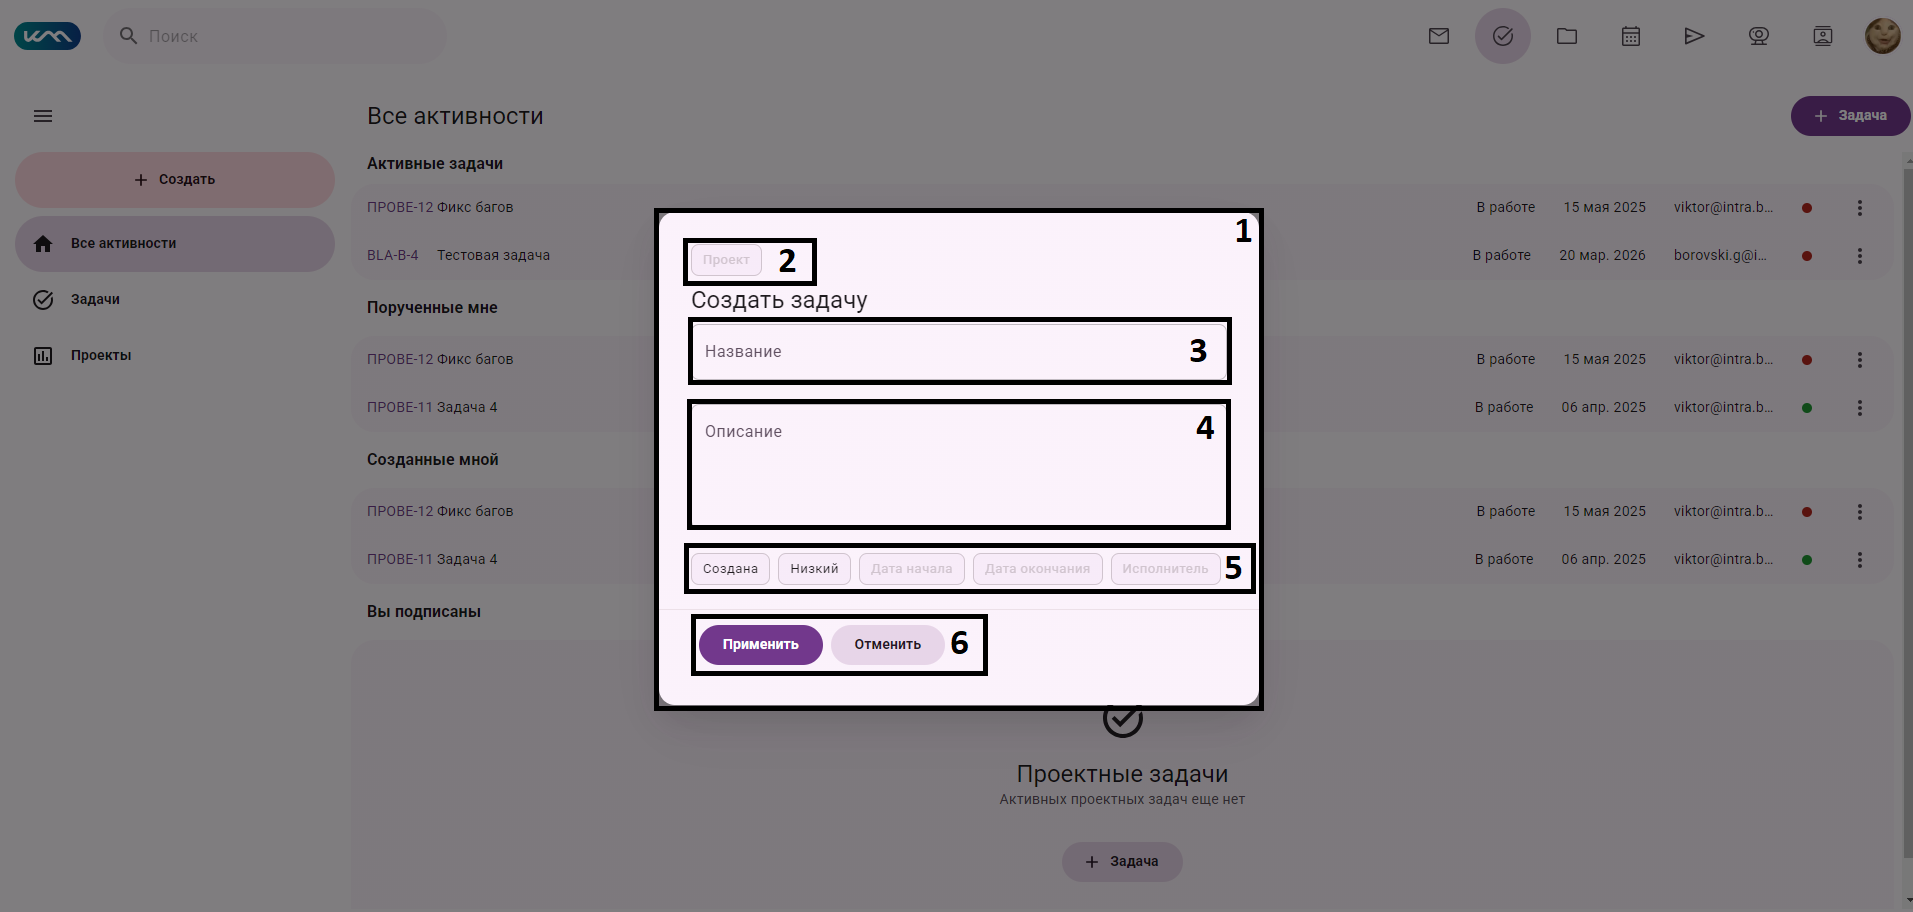
\includegraphics[width=1\linewidth]{images/проекты3}
	\caption{Композиция интерфейса создания задачи}
	\label{templ:image7c}
\end{figure}

Композиция интерфейса просмотра задачи в сервисе <<Проекты>> представлена на рисунке \ref{templ:image7d} и состоит из:
\begin{itemize}
  \item всплывающего окна (1);
  \item кнопок для отслеживания, удаления и архивирования задачи (2);
  \item подробной информации о задаче (3);
  \item кнопок для прикрепления файлов/ссылок, добавление подзадачи (4);
  \item раздела с комментариями (5);
  \item поля для ввода комментария (6);
  \item кнопки для отправки комментария (7);
\end{itemize}
\begin{figure}[H]
	\centering
	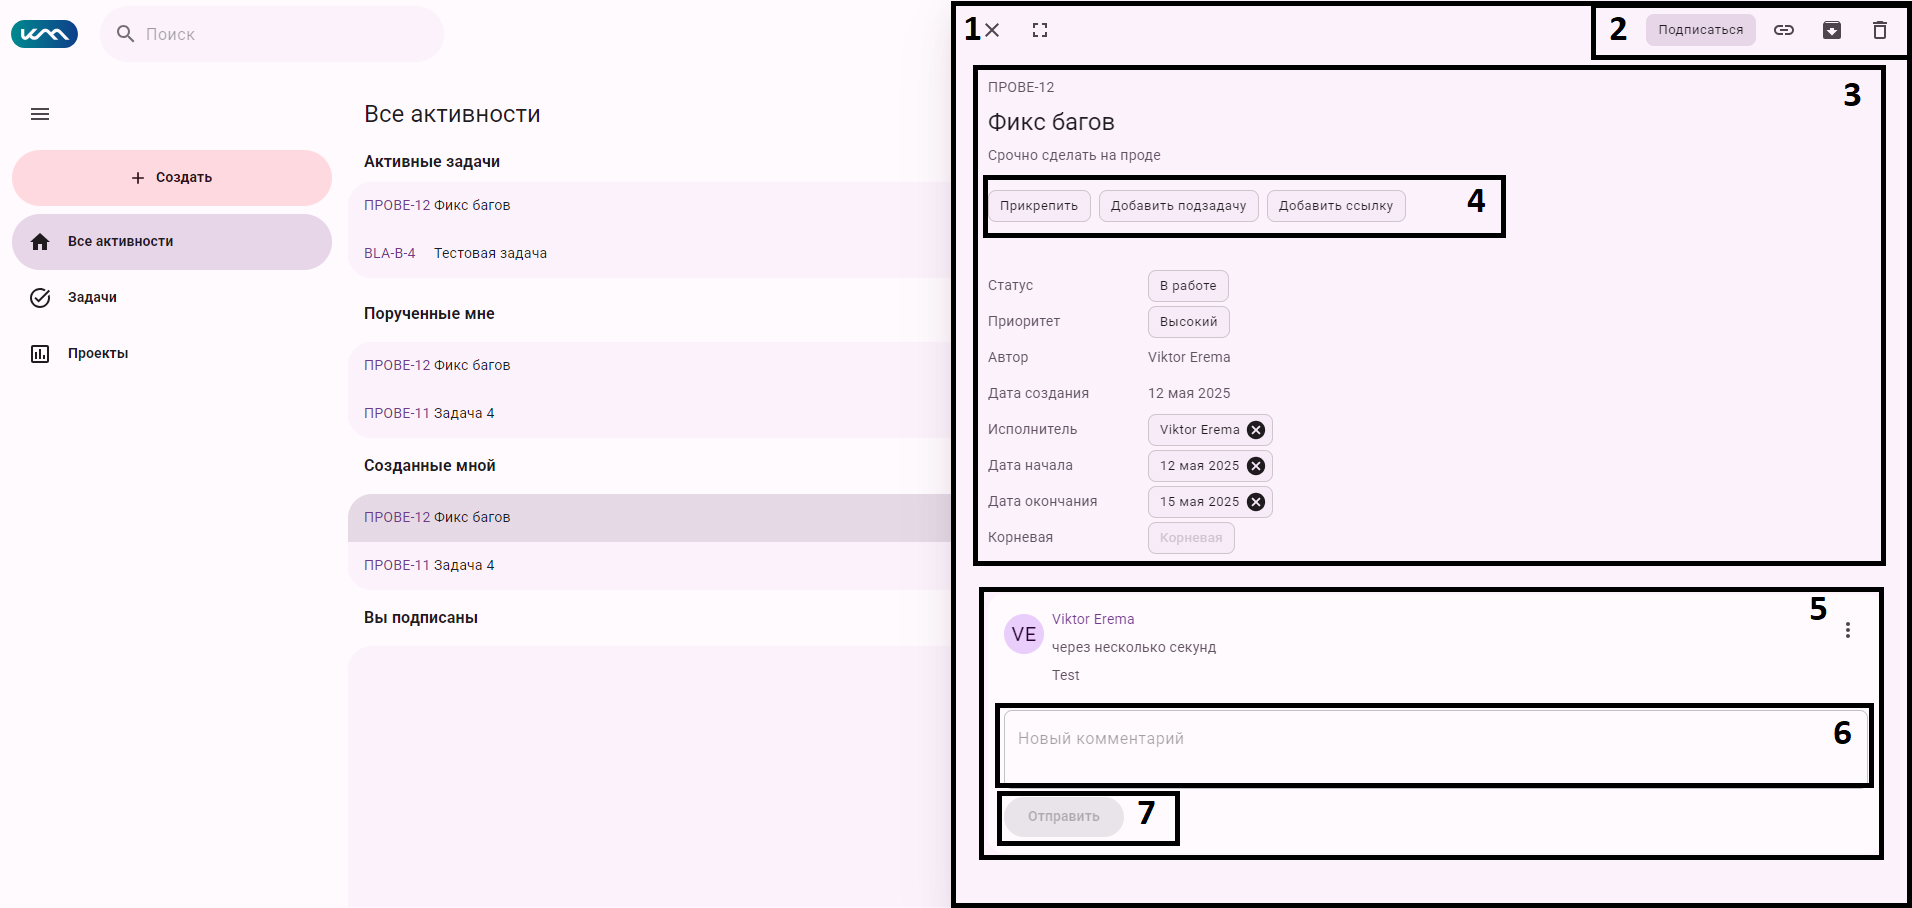
\includegraphics[width=1\linewidth]{images/проекты4}
	\caption{Композиция интерфейса просмотра задачи}
	\label{templ:image7d}
\end{figure}

Композиция интерфейса сервиса <<Разговоры>> представлена на рисунке \ref{templ:image8} и состоит из:
\begin{itemize}
  \item компонента навигации по сервисам (1);
  \item кнопки для создания комнаты (2);
  \item списка комнат (3);
  \item кнопки для создания диалога (4);
  \item кнопки для создания канала (5);
  \item окна для работы с комнатой (6);
  \item поля для написания сообщения (7);
\end{itemize}
\begin{figure}[H]
	\centering
	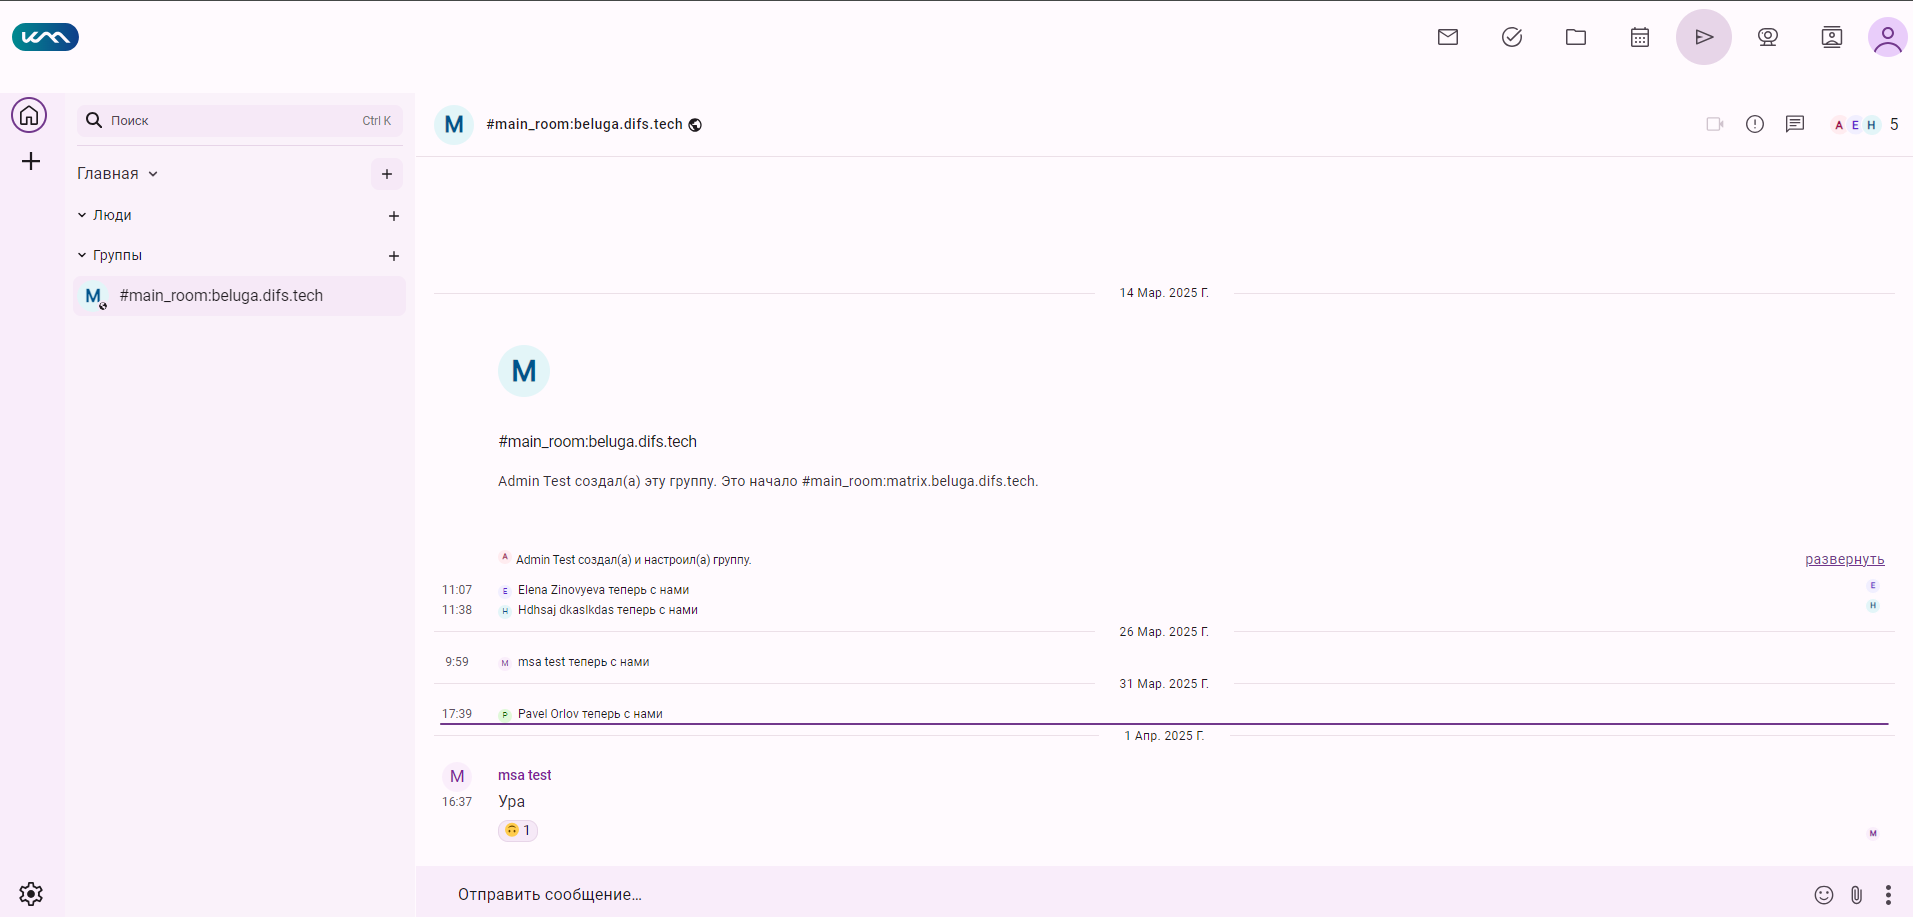
\includegraphics[width=1\linewidth]{images/разговоры}
	\caption{Композиция интерфейса сервиса <<Разговоры>>}
	\label{templ:image8}
\end{figure}

Композиция интерфейса сервиса <<Файлы>> представлена на рисунке \ref{templ:image9} и состоит из:
\begin{itemize}
  \item компонента навигации по сервисам (1);
  \item кнопки для создания папки/загрузки файла в текущую папку (2);
  \item списка папок (3);
  \item окна для работы с файлами (4);
  \item кнопки для перехода в настройки сервиса (5);
\end{itemize}
\begin{figure}[H]
	\centering
	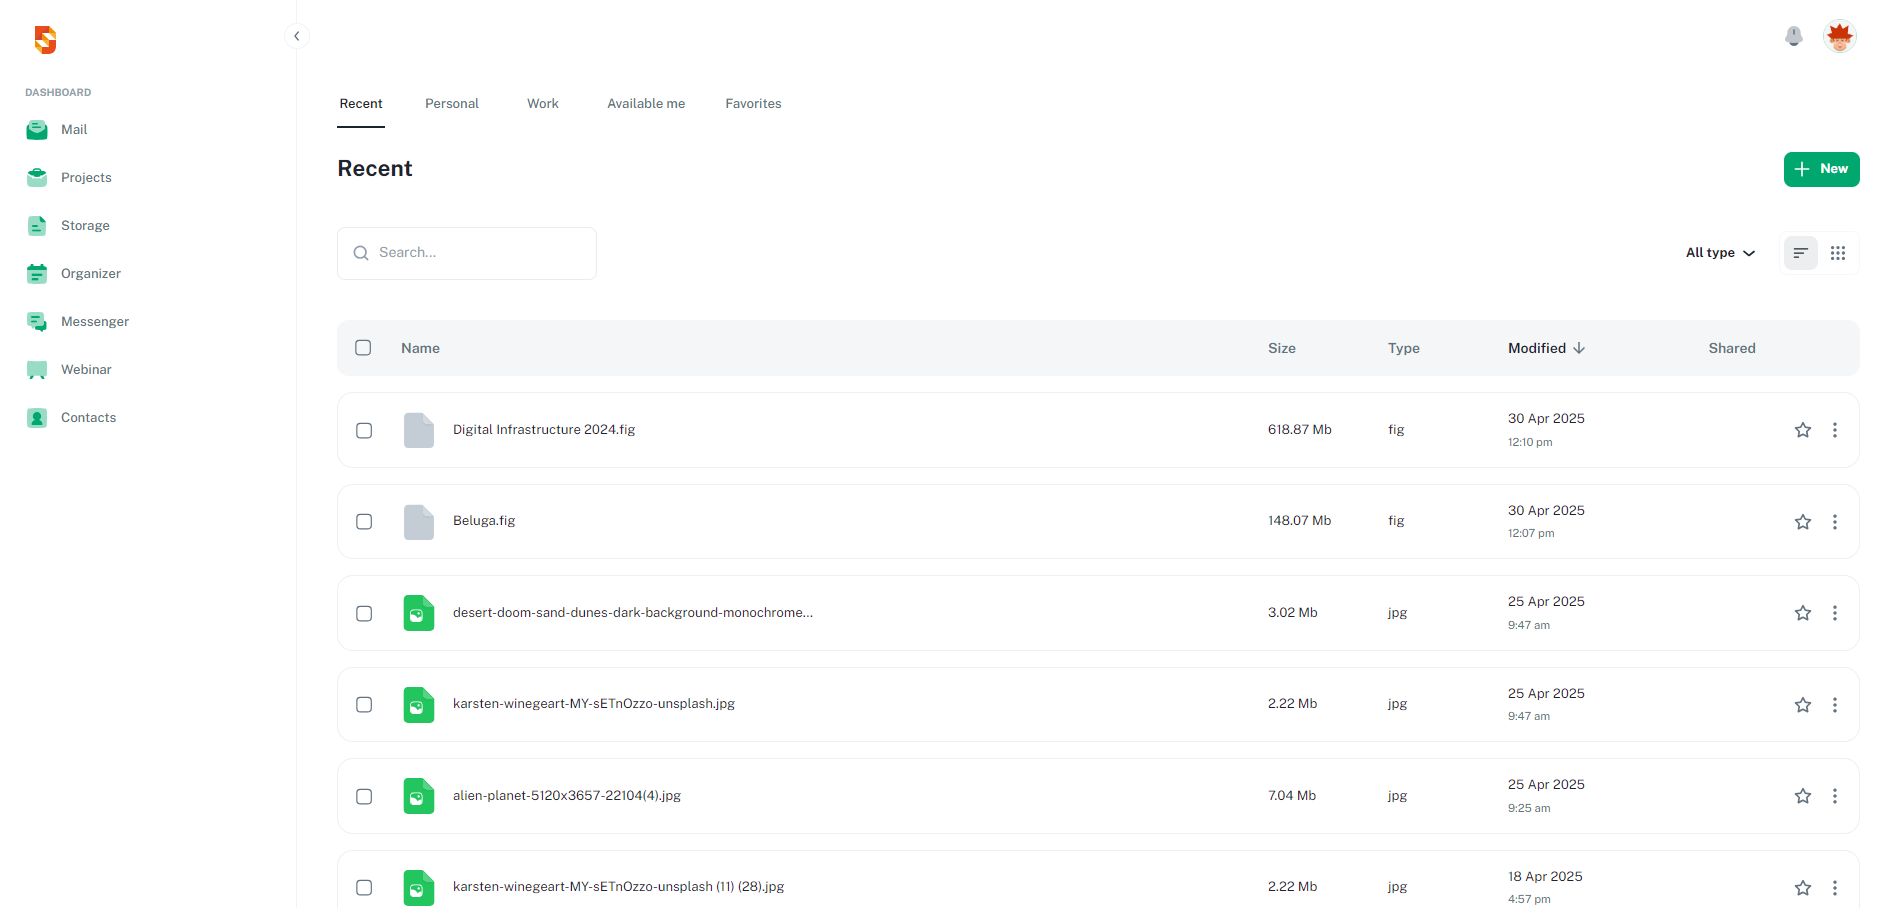
\includegraphics[width=1\linewidth]{images/файлы}
	\caption{Композиция интерфейса сервиса <<Файлы>>}
	\label{templ:image9}
\end{figure}

Композиция интерфейса создания файла в сервисе <<Файлы>> представлена на рисунке \ref{templ:image9b} и состоит из:
\begin{itemize}
  \item всплывающего окна (1);
  \item поля для ввода названия файла (2);
  \item кнопок действий (3);
\end{itemize}
\begin{figure}[H]
	\centering
	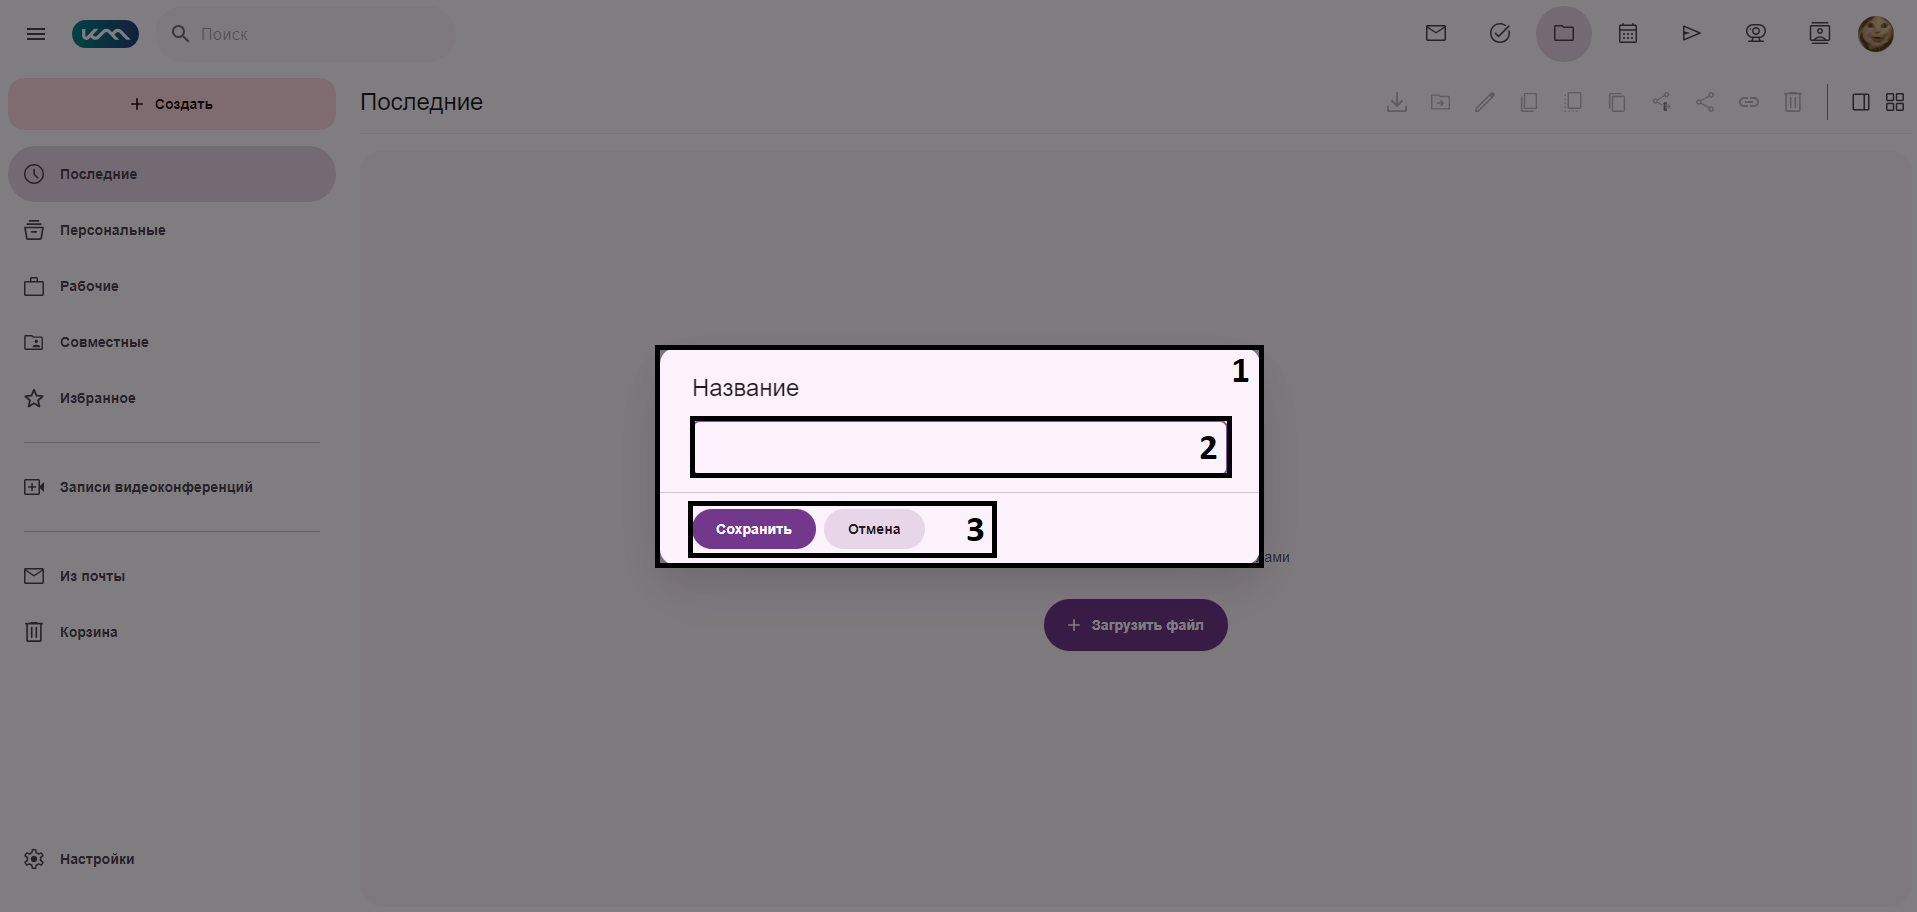
\includegraphics[width=1\linewidth]{images/файлы2}
	\caption{Композиция интерфейса создания файла}
	\label{templ:image9b}
\end{figure}

Композиция интерфейса загрузки файла в сервисе <<Файлы>> представлена на рисунке \ref{templ:image9c} и состоит из:
\begin{itemize}
  \item всплывающего окна (1);
  \item поля для выгрузки файла (2);
  \item кнопок действий (3);
\end{itemize}
\begin{figure}[H]
	\centering
	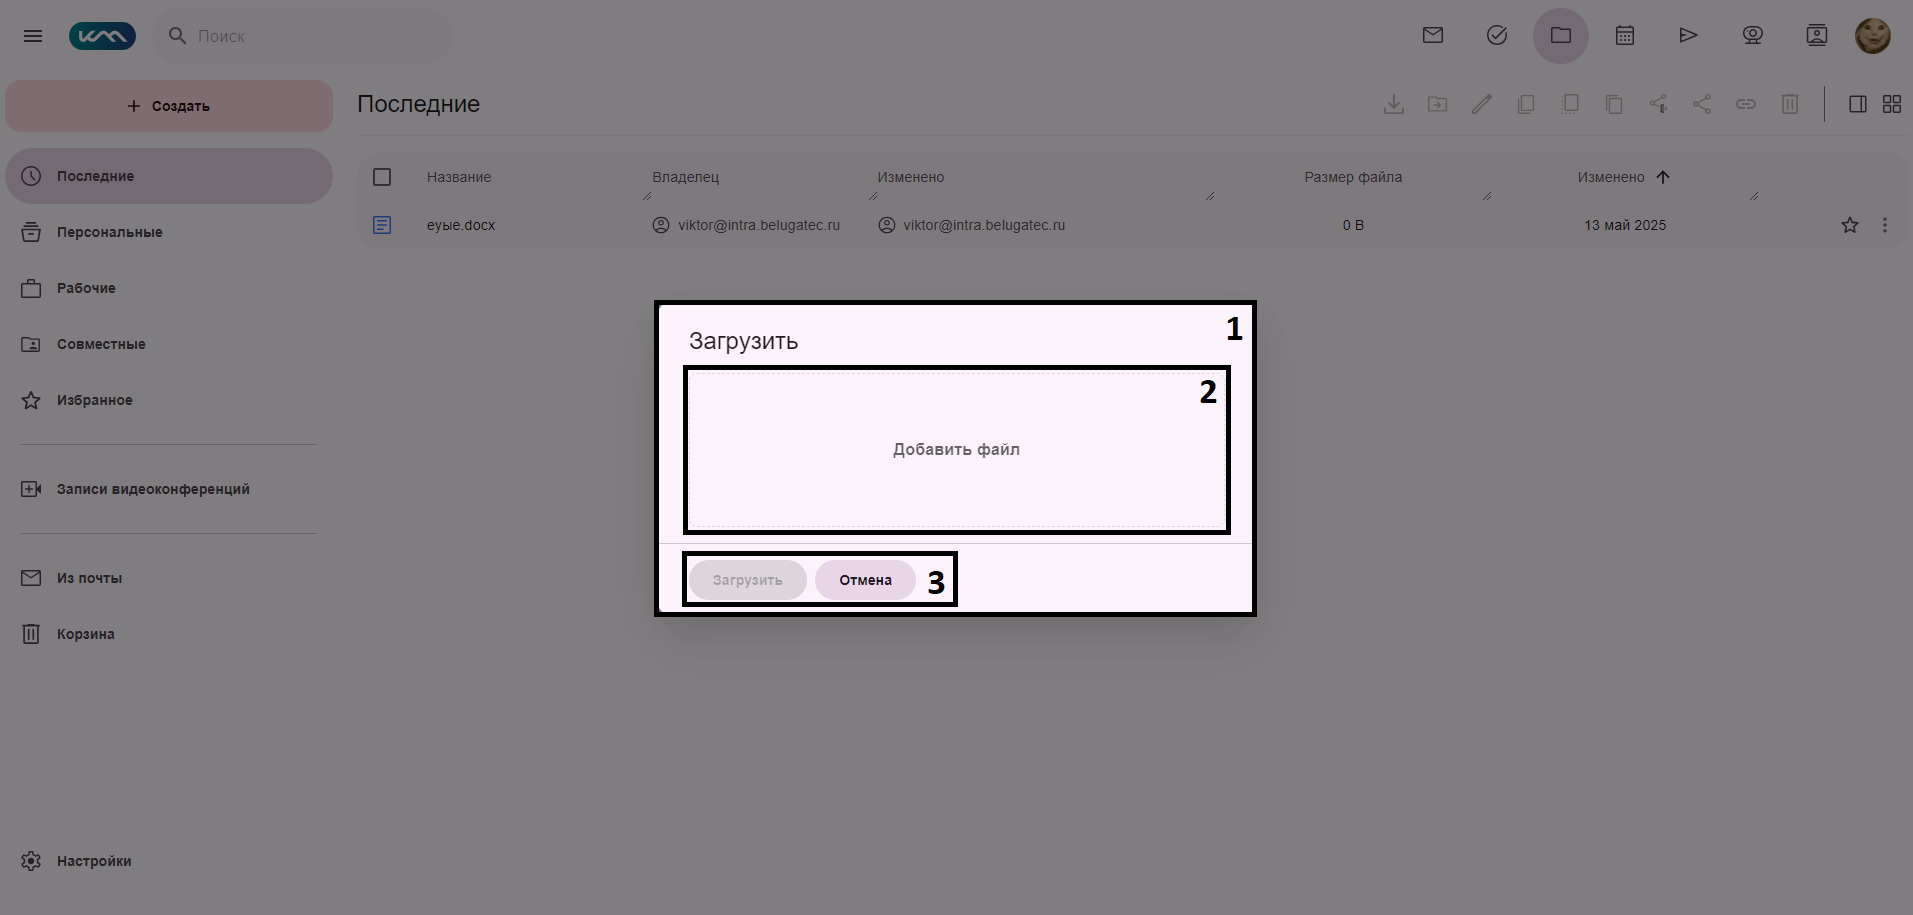
\includegraphics[width=1\linewidth]{images/файлы3}
	\caption{Композиция интерфейса загрузки файла}
	\label{templ:image9c}
\end{figure}

Композиция интерфейса создания папки в сервисе <<Файлы>> представлена на рисунке \ref{templ:image9d} и состоит из:
\begin{itemize}
  \item всплывающего окна (1);
  \item поля названия папки (2);
  \item кнопок действий (3);
\end{itemize}
\begin{figure}[H]
	\centering
	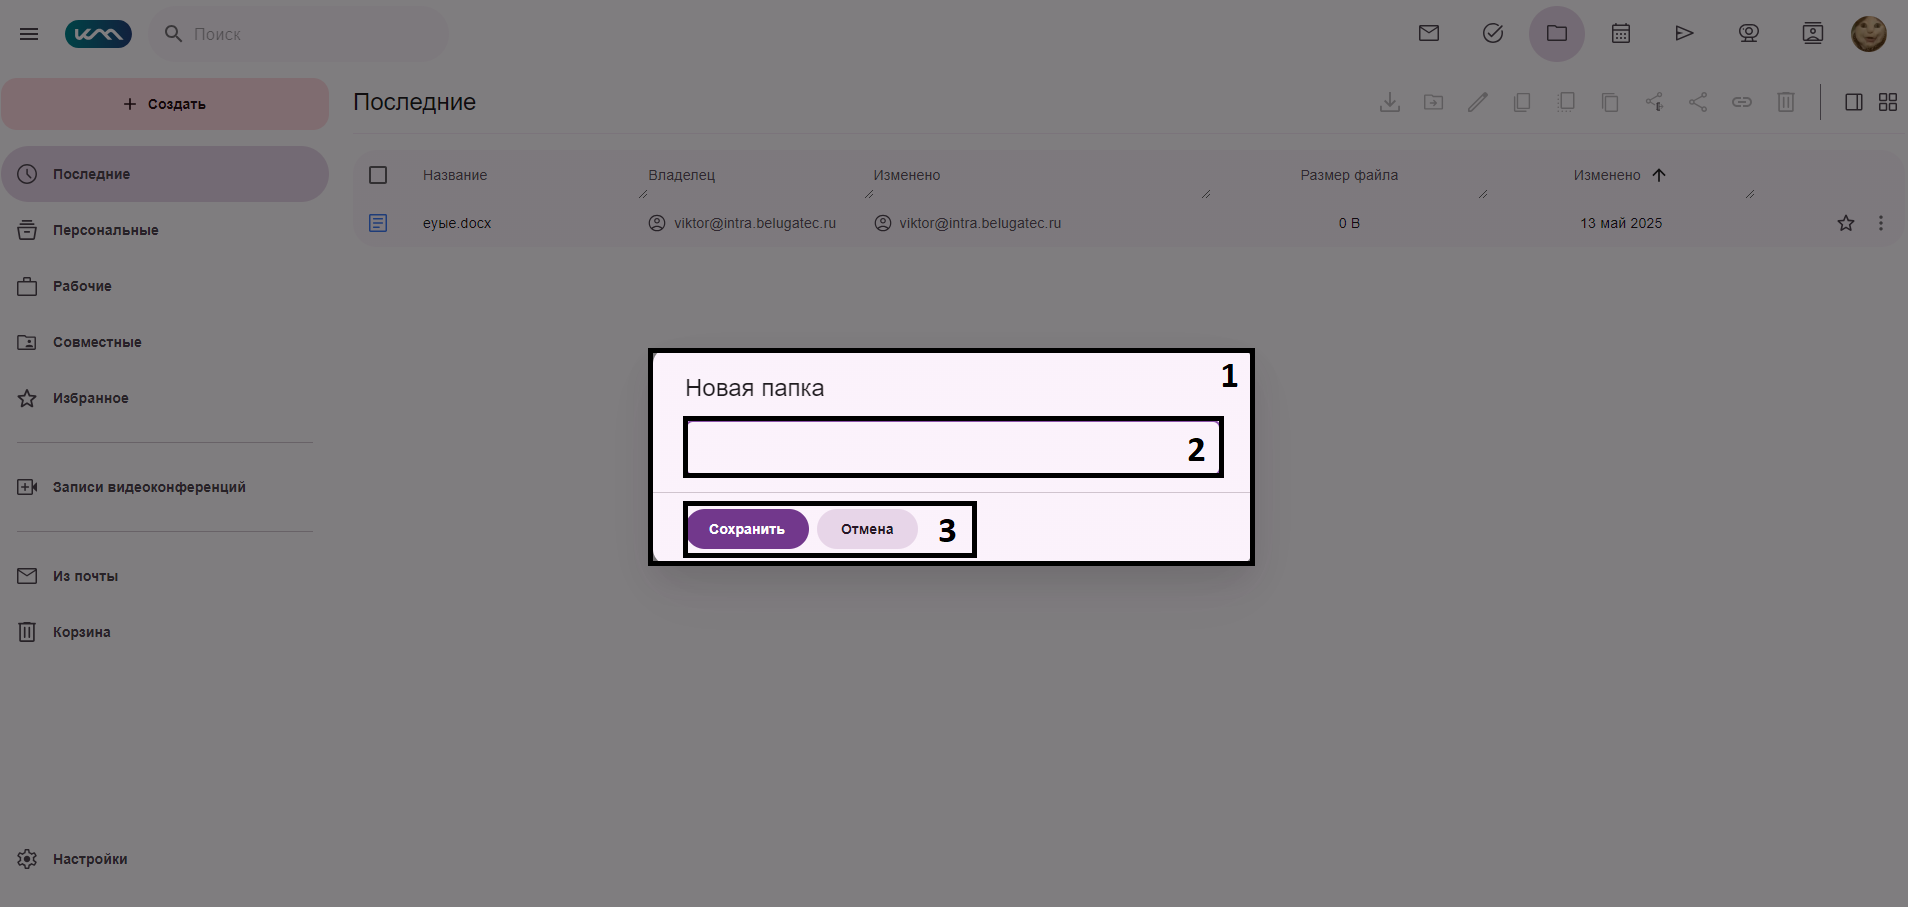
\includegraphics[width=1\linewidth]{images/файлы4}
	\caption{Композиция интерфейса создания папки}
	\label{templ:image9d}
\end{figure}

\clearpage
\subsection{Моделирование вариантов использования}

Для разрабатываемой системы была создана модель, которая демонстрирует способы взаимодействия пользователей с программой с помощью унифицированного языка моделирования UML.

На диаграмме вариантов использования система представлена через набор сценариев (прецедентов), с которыми взаимодействуют актёры — пользователи или внешние компьютерные системы. Каждый вариант использования отображается в виде овала с подписью, обозначающей соответствующий сценарий. Эти сценарии описывают, как пользователь может достичь своих целей, взаимодействуя с функциональностью программы. Взаимосвязь между актёрами и вариантами использования показывается через ассоциации.

Применение UML-диаграмм для визуализации работы системы помогает выявить основные взаимодействия и зависимости между компонентами, что облегчает понимание требований, упрощает проектирование и способствует более качественной разработке и тестированию программного обеспечения.

Пользователь с ролью сотрудника имеет доступ ко всем функциональным модулям веб-платформы:
\begin{enumerate}
  \item Работа с сервисом <<Почта>>.
  \item Работа с сервисом <<Разговоры>>.
  \item Работа с сервисом <<Проекты>>.
  \item Работа с сервисом <<Календарь>>.
  \item Работа с сервисом <<Видеоконференцсвязь>>.
  \item Работа с сервисом <<Файлы>>.
  \item Работа с сервисом <<Контакты>>.
  \item Работа с сервисом <<Настройки>>.
  \item Работа с сервисом <<Панель управления>>.
\end{enumerate}
Эти действия отображены на диаграмме прецедентов, представленной на рисунке~\ref{templ:actor1}.
\begin{figure}[H]
	\centering
	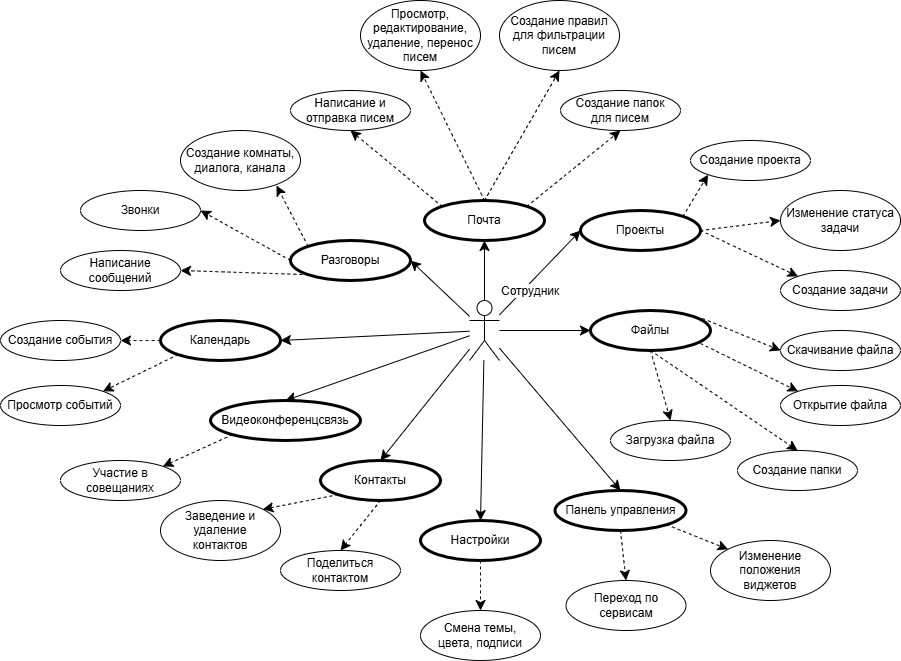
\includegraphics[width=1\linewidth]{images/umldi}
	\caption{Диаграмма прецедентов для сотрудника}
	\label{templ:actor1}
\end{figure}

\subsection{Требования к оформлению документации}

Документация проекта и программного продукта должна оформляться в соответствии с ГОСТ 19.102–77 и ГОСТ 34.601–90. Используемая терминология должна соответствовать принятой в сфере ИТ и быть однозначно понятной.
